%                         lezione 8 parte 2

\chapter{Omologia cellulare}

\section{CW-complessi}

Considero $ \Disk{n} $, vale che $ \partial\Disk{n} = \Sph{n-1} $, considerato lo spazio quoziente
$ X = \quot{\Disk{n}}{\partial \Disk{n}} $, questo è il quoziente del disco per la relazione
di equivalenza che fa collassare il bordo in un punto $ p $. Si trova che $ X \simeq \Sph{n} $.
In 2 dimensioni questo si visualizza facilmente: considerato il cerchio, si spinge il centro
in basso in modo da ottenere una superficie semisferica, quindi indentificare tutti i punti
del bordo con un unico punto vuol dire chiudere il cerchio ottenendo qualcosa di simile ad
una goccia, che è omeomorfa ad una sfera. In pratica quello che ho fatto è:
definisco $ X^{(0)} = P = \set{p} $ e $ \phi \colon \Sph{n-1} \to X^{(0)} $, posso definire:
\[
  X^{(1)} = X^{(0)} \cup_\phi \Disk{n}
\]
Dove con $ \cup_\phi $ si intende, con $ X, Y $ spazi topologici:
\newmathsymb{disgun}{\sqcup}{Unione disgiunta}
\[
  X^{(0)} \cup_\phi \Disk{n} = \quot{X^{(0)} \sqcup \Disk{n}}{p \sim \phi(q)} \quad \forall q \in \Sph{n-1}
\]
Quello che sto facendo in pratica è prendendo un punto e un disco, quindi
identifico il bordo del disco con il punto.

% Considero la proiezione al quoziente $ \pi \colon \Disk{n} \to \Sph{n} $
% con $ \Sph{n} \cong X^{(0)} \cup_\phi \Disk{n} $.

\begin{definition}
  Si dice che lo spazio topologico $ X $ è un \textbf{CW-complesso} di tipo finito\index{CW-complesso},
  dove C singif>>>>>>>>>>>ica \emph{closure finite} e W \emph{weak topology} se è dato dai seguenti oggetti topologici:
  \begin{enumerate}
  \item Un insieme finito $ X^{(0)} = \set{p_1, \dots, p_n} $ detto \textbf{$ 0 $-scheletro}\index{$ 0 $-scheletro}
  \item Il \textbf{$ k $-scheletro}\index{$ k $-scheletro} $ X^{k} $ si costruisce induttivamente
    a partire da $ X^{(k-1)} $ attaccando opportunamente dei dischi nel modo seguente.
    Considero un numero finito di dischi $ k $-dimensionali $ \Disk{k}_\alpha $,
    detti \textbf{celle}\index{Cella} (o cella chiusa, mentre
    il loro interno è detto cella aperta) per ciascuno si definice una mappa
    continua di attaccamento $ \phi_\alpha \colon \partial\Disk{k}_\alpha \to X^{(k-1)} $, quindi si definisce:
    \[
      X^{(k)} = X^{(k-1)} \cup_\phi \bigcup_\alpha \Disk{k}_\alpha = \quot{ X^{(k-1)} \sqcup \Disk{k}_\alpha}{x \sim \phi_\alpha(x)} \quad \forall \alpha \text{ e }
      \forall x \in \partial \Disk{k}_\alpha
    \]
  \item Esiste $ N \in \mathbb{N} $ tale che $ X^{(0)} \subseteq X^{(1)} \subseteq \dots \subseteq X^{(N)} =: X $
  \end{enumerate}
\end{definition}

Si dimostra che in generale la cella chiusa non è omeomorfa all'immagine, mentre la cella
aperta lo è.

In generale uno spazio ha numerose strutture di CW complesso.

La topologia è detta debole perché la topologia di unione disgiunta per tutti i $ k $-scheletri,
e questo è la topologia più debole di tutte. In questa topologia un insieme è aperto in $ X $
se e solo se è aperto la sua intersezione con tutti gli $ X^{(i)} $ è aperta.

\begin{example}[Sfere]
  $ \Sph{n} $ per $ n \geq 1 $ ammette una struttura di CW complesso: sia $ X^{(0)} = \set{p} $ con
  $ p \in \Sph{n} $ e sia $ \phi \colon \partial \Disk{n} \to \set{p} $ mappa costante, allora
  $ \Sph{n} = X^{(0)} \cup_\phi \Disk{n} = \quot{\Disk{n}}{\partial \Disk{n}} $, cioè una $ 0 $-cella e una
  $ n $-cella.

  Alternativamente una seconda possibile struttura è: considero l'equatore di $ \Sph{n} $ che
  è uno $ \Sph{n-1} $ su questo attacco due dischi che sono calotta superiore e inferiore.
  $ X^{(0)} = \set{p_1, p_2} $ e $ X^{(1)} = \Disk{1}_1 \cup \Disk{1}_2 $, quindi le mappe
  sono:
  \begin{gather*}
    \phi_1 \colon \partial \Disk{1}_1 \to X^{(0)} \quad \text{cioè} \quad \phi_1 \colon \set{-1, +1} \to \set{p_1, p_2} \\
    \phi_1 \colon \partial \Disk{1}_2 \to X^{(0)} \quad \text{cioè} \quad \phi_2 \colon \set{-1, +1} \to \set{p_1, p_2}
  \end{gather*}
  Quindi deve essere:
  \[
    \phi_1(1) = p_1 \quad \phi_1(-1) = p_2 \qquad  \phi_2(1) = p_2 \quad \phi_2(-1) = p_1
  \]
  A questo punto $ X^{(1)} \cup_\phi (\Disk{1}_1 \cup \Disk{1}_2) = \Sph{1} $ e si può aggiungere
  $ \Disk{2} $, cioè $ X^{(2)} = \Disk{2}_1 \cup \Disk{2}_2 $, ora:
  \begin{gather*}
    \psi_1 \colon \partial \Disk{2}_1 \to X^{(2)} \\
    \psi_1 \colon \partial \Disk{2}_2 \to X^{(0)}
  \end{gather*}
  Cioè $ \psi_j \colon \Sph{1} \to X^{(1)} $, quindi $ \psi_j \colon \Sph{1} \to \Sph{1} $ e quindi si può prendere
  l'identità. Si ottiene così una $ 2 $-sfera. A questo punto si può procedere ad libidum.
\end{example}

\begin{example}[Toro]
  Considerato un toro $ T = \Sph{1} \times \Sph{1} $ una possibile costruzione si basa sul prendere
  come punti $ p $ i vertici del quadrato dal quale si fanno le identificazioni per ottenere il
  toro. $ X^{(0)} = \set{p} $, ho quindi due lacci. Quindi:
  \[
    X^{(1)} = (\Disk{1}_1 \cup \Disk{1}_2) \cup_\phi X^{(0)}
  \]
  Le mappe:
  \begin{gather*}
    \phi_1 \colon \set{-1, +1} \to \set{p} \\
    \phi_2 \colon \set{-1, +1} \to \set{p}
  \end{gather*}
  La cella è $ X^{(2)} = (\Disk{2} \cup_\psi X^{(1)}) $ con $ \psi \colon \Sph{1} \to X^{(1)} $
  [MANCA IL SECONDO MODO]
\end{example}

\begin{definition}
  Si definice lo \textbf{spazio proiettivo reale}\index{Spazio proiettivo reale} $ \mathbb{P}^n(\RN{}) = \quot{\RN{n+1} \setminus \set{0}}{\sim} $
  con $ \vec{x} \sim \vec{y} $ se e solo se $ \vec{x} $ e $ \vec{y} $ sono multipli,
  cioè se esiste $ \lambda \in \RN{+} $ tale che $ \vec{x} = \lambda \vec{y} $.
\end{definition}

Si dimostra che $ \mathbb{P}^n(\RN{}) \cong \quot{\Sph{n}}{H} $ con $ H = \set{\Id{\Sph{n}}, a_{\Sph{n}}} $.

Si trova che:
\begin{itemize}
\item $ \mathbb{P}^1(\RN{}) = \Sph{1} = \RN{} \cup {\infty} $
\item $ \mathbb{P}^2(\RN{}) = \mathbb{P}^1(\RN{}) \cup_\phi \Disk{2} $
  Ho $ \quot{\Sph{2}}{H} $, l'emisfero sud della sfera si identifica con quello
  nord per l'applicazione di antipodalità.
  $ \phi = a \big \lvert_{\Sph{1}} $ e $ \Sph{1} = \mathbb{P}^1(\RN{}) $ e $ \Sph{1} = \partial \Disk{2} $,
  quindi:
  \begin{align*}
    \phi \colon \Sph{1} & \to \Sph{1} \\
    (x,y) & \mapsto (-x,-y)
  \end{align*}
\item Se considero $ \mathbb{P}^2(\RN{}) \cup_\phi \Disk{3} $ con:
  \[
    \phi \colon \partial \Disk{3}  \to \mathbb{P}^2(\RN{})
  \]
  cioè il passaggio al quoziente:
  \[
    \phi \colon \Sph{2}  \to \quot{\Sph{1}}{H}
  \]
\end{itemize}

\begin{example}[Spazi proiettivi]
  Se $ X^{(k)} = \mathbb{P}^k(\RN{}) \cup_\phi \Disk{k+1} $ con
  \[
    \phi \colon \partial \Disk{k+1}  \to \mathbb{P}^k(\RN{})
  \]
  Cioè:
  \[
    \phi \colon \Sph{k}  \to \mathbb{P}^k(\RN{})
  \]
  Cioè scelgo $ \phi $ come la proiezione sul quoziente da $ \Sph{k} $ a $ \mathbb{P}^k(\RN{}) = \quot{\Sph{k+1}}{H} $,
  questo è uno spazio compatto.
  $ \mathbb{P}^k(\RN{}) $ è uno spazio di Hausdorf, voglio mostrare che $ X^{(k+1)} \cong \mathbb{P}^{k+1}(\RN{}) $.
  Cerco un'applicazione continua biunivoca e chiusa $ \Phi \colon X^{(k+1)} \to  \mathbb{P}^{k+1}(\RN{}) $,
  cioè un omeomorfismo. Ho il digramma:
  \[
    \begin{tikzcd}
      \mathbb{P}^{k}(\RN{}) \sqcup \Disk{k+1} \arrow{r}{\eta} \arrow{d}{} &  \mathbb{P}^{k+1}(\RN{}) \\
      X^{(k+1)} \arrow{ru}{\Phi}
    \end{tikzcd}
  \]
  \begin{exercise}
    Dimostrare che $ \eta $ è continua e gode di tutte le buone proprietà.
  \end{exercise}
  So che $ i \colon  \mathbb{P}^{k}(\RN{}) \incl \mathbb{P}^{k+1}(\RN{}) $ (è un iperpiano all'infinito),
  quindi posso usare l'inclusione.

  Devo trovare una mappa $ j \colon \Disk{k+1} \to \mathbb{P}^{k+1}(\RN{}) $. $ i $ è ovvia:
  $ i([z_0, \dots, z_k]) = [z_0, \dots, z_k; 0] $, mentre $ j $:
  \[
    j \colon [z_0, \dots, z_k] \mapsto  \left[z_0, \dots, z_{k+1} = \sqrt{1 - \sum_{j=1}^k z_i^2}\right]
  \]
  Siccome $ \sum_{j=1}^k z_i^2 \leq 1 $ l'applicazione è ben definita, quindi $ \eta = (i,j) $.
\end{example}




    %     lezione 8

\section{Congettura di Poincaré}

Ho calcolato l'omologia di una sfera generica:
\[
  H_k(\Sph{n}) \cong
  \begin{cases}
    \Z & \text{ se } k \in \set{0,n} \\
    0 & \text{ se } k \not \in \set{0,n}
  \end{cases}
\]
In particolare ho $ H_0(\Sph{n}) \cong \Z $ ed è generato dalla classe di
omologia di un punto qualsiasi, mentre $ H_n(\Sph{n}) \cong \Z $ è generatodalla
classe di omologia di un $ n $-simplesso singolare $ \tau_n \colon \Delta_n \to \Sph{n} $.

Per $ n = 2 $ ho $ \Sph{2} $ è una $ 2 $-varietà topologica compatta e connessa
il cui gruppo fondamentale è banale e i gruppi di omologia noti.

\begin{proposition}
  Se $ \M $ è una $ 2 $-varietà topologica compatta e connessa tale che $ \forall k \geq 2 $
  $ H_k(\M) \cong H_k(\Sph{2}) $ allora $ \M \simeq \Sph{2} $.
\end{proposition}
\begin{proof}
  Esiste un teorema di classificazione delle varietà topologiche di dimensione $ 2 $
  compatte e connesse, questo dice che $ \M \simeq V_g $ oppure $ \M \simeq U_n $.
  Dove:
  \[
    V_g =
    \begin{cases}
      \Sph{2} & \text{se } g = 0 \\
      \quot{P_{4g}}{\sim} & \text{se } g \geq 1
    \end{cases}
  \]
  Dove $ \sim $ è l'identificazione $ a_1 b_1 a_1^{-1}b_1^{-1}\dots a_g b_g a_g^{-1}b_g^{-1} $,
  come ad esempio il toro, mentre:
  \[
    U_n =
    \begin{cases}
      \mathbb{P}^2(\RN) & \text{se } n = 0 \\
      \quot{P_{2g}}{\sim} & \text{se } n \geq 1
    \end{cases}
  \]
  Con $ \sim $ è l'identificazione $ a_1 a_1 \dots a_n a_n $, come ad esempio
  la bottiglia di Klein.
  Tutti i $ V_g $ non sono omeomorfi tra loro, e similmente gli $ U_n $, e neppure
  gli $ U_n $ e i $ V_g $ sono vicendevolmente omeomorfi in quanto i primi sono
  non orientabili, mentre i secondi si.

  Ho calcolato:
  \[
    H_1(V_g) \cong
    \begin{cases}
      H_1(\Sph{2}) & \text{se } g = 0 \\
      \Z^{2g} & \text{se } g \geq 1
    \end{cases}
  \]
  $ V_g $ con $ g \geq 1 $ non hanno lo stesso tipo di omologia di $ \Sph{2} $ perché
  $ H_1(V_g) $ è non banale, mentre il gruppo fondamentale di $ \Sph{2} $ lo è.
  Similmente $ H_1(\mathbb{P}^2(\RN)) \cong \pi_1(\mathbb{P}^2(\RN)) \cong \Z_2 $, che non è
  banale, e $ H_1(U_n) \cong \Ab{\pi_1(U_n)} $, ma per Seifert-van Kampen:
  \[
    \pi_1(U_n) = \langle a_t, \dots, a_n \; | \; a_1^2\dots a_n^2 = 1 \rangle \Rightarrow \Ab{\pi_1(U_n)} = \langle a_t, \dots, a_n, c = a_1 \dots a_n \; | \; a_1^2\dots a_n^2 = 1 \rangle =
    \Z_2 \oplus \Z^{n-1}
  \]
  Dove $ \Z_2 $ viene dal fatto che abelianizzando $ a_1^2\dots a_n^2 = (a_1 \dots a_n)^2 = 1 $ quindi
  $ c = \pm 1 $, mentre $ \Z^{n-1} $ è il gruppo libero generato dai rimanenti.
  Questo non è banale, quindi l'unico spazio possibile è proprio $ \Sph{2} $.
\end{proof}

Cosa si può invece dire su $ \Sph{3} $? Vale la seguente proposizione:
\begin{proposition}
  Se $ \M $ è una $ 3 $-varietà topologica compatta e connessa tale che $ \forall k \geq 3 $
  $ H_k(\M) \cong H_k(\Sph{3}) $ allora non si può concludere che $ \M \simeq \Sph{3} $.
\end{proposition}
\begin{proof}
  Costruisco un controesempio, noto come \textbf{spazio dodecaedrico di Poincaré}\index{Spazio dodecaedrico},
  o anche spazio a omologia razionale\index{Spazio a omologia razionale ! \vedi{Spazio dodecaedrico}}.
  Costruisco $ P $ $ 3 $-varietà topologica compatta e connessa con lo stesso tipo di omologia di
  una $ 3 $-sfera ma non omeomorfa a $ \Sph{3} $ in quanto il gruppo fondamentale è finito
  non abeliano di ordine 120.
  Parto da $ \Sph{3} $, posso scrivere:
  \[
    \Sph{3} \subseteq \mathbb{C}^2 \qquad \Sph{3} = \set{ (z_0, z_1) \in \mathbb{C}^2 | |z_0|^2 + |z_1|^2 = 1}
  \]
  Infatti $ z_0 = x + i y $ e $ z_1 = t + i w $ quindi $ |z_0|^2 = (x + iy)(x - iy) = x^2 + y^2 $
  e $ |z_0|^2 = (t + iw)(t - iw) = t^2 + w^2 $ e quindi ottengo:
  \[
    \Sph{3} = \set{ (x,y,t,w) \in \RN{4} | x^2 + y^2 + t^2 + w^2 = 1}
  \]
  Così come $ \Sph{1} $ ha una struttura di gruppo U(1) è possibile strutturare
  $ \Sph{3} $ come gruppo SU(2):
  \[
    \mathrm{SU(2)} = \set{A \in M_2(\mathbb{C}) | \det{A} = 1, \; AA^\dagger = \Id{2}}
  \]
  Quindi $ \mathrm{SU(2)} \subseteq \mathbb{C}^4 $, si dimostra che $ A \in \mathrm{SU(2)} $ se e solo se
  è della forma:
  \[
    \begin{pmatrix}
      \alpha & - \beta^\star \\
      \beta & \alpha^\star \\
    \end{pmatrix}
    \text{ con } \alpha,\beta \in \mathbb{C} \text{ e } |\alpha|^2 + |\beta|^2 = 1
  \]
  Quello che sto dicendo è che i vettori in $ \mathbb{C}^2 $ $ (\alpha, \beta) $ e $ (-\beta^\star, \alpha^\star) $ sono
  normalizzati e sono tra di loro ortogonali.

  Si costruisce immediatamente la corrispondenza buinivoca tra SU(2) e $ \Sph{3} $:
  \begin{align*}
    \mathrm{SU(2)} & \leftrightarrow \Sph{3} \\
    \begin{pmatrix}
      \alpha & - \beta^\star \\
      \beta & \alpha^\star \\
    \end{pmatrix} & \leftrightarrow (\alpha,\beta)
  \end{align*}
  In questo modo si può definire un prodotto su $ \Sph{3} $ rappresentanto
  $ x,y,t,w $ come numeri complessi e passando alla controparte matriciale, dove
  il prodotto è definito naturalmente come prodotto riga per colonna, quindi
  una volta svolto il prodotto si torna alla notazione a quattro reali. A questo
  punto è triviale trovare l'identità e l'elemento inverso che permettono di dare
  a $ \Sph{3} $ la struttura di gruppo.

  SU(2) può essere visto come spazio topologico con topologia indotta da $ \mathbb{C}^4 $,
  in questo senso SU(2) e $ \Sph{3} $ sono sia isomorfi come gruppi che omeomorfi
  come spazi topologici.

  La costruzione dello spazio dodecaedrico si basa sulle isometrie del dodecaedro $ D_{12} $,
  questo è un solido regolare con 12 facce, 30 spigoli e 20 vertici.
  Il gruppo di isometrie del dodecaedro, cioè:
  \[
    \mathrm{Isom}(D_{12}) = \set{ g \colon \RN{3} \to \RN{3} | g \text{ regolare e } g(D_{12}) = D_{12}}
  \]
  Questo gruppo si può vedere come:
  \[
    \mathrm{Isom}(D_{12}) \cong A_5 \times \Z_2
  \]
  Dove $ A_5 $ è un sottogruppo di $ \mathrm{Isom}(D_{12}) $ ed è il gruppo
  alterno (cioè il gruppo delle permutazioni pari) su 5 elementi e quindi ha ordine 60.
  Le 60 trasformazioni che sono in $ A_5 $ sono l'identità, 24 rotazioni di $ \frac{2}{5} \pi $ attorno
  agli assi per i centri di facce opposti, 20 rotazioni di $ \frac{2}{3} \pi $ attorno
  agli assi per vertici opposti e 15 rotazioni di $ \pi $ attorno agli assi per
  i punti medi di spigoli opposti.
  $ \Z_2 $ invece è dovuto all'applicazione antipodale che è $ (x,y,z) \mapsto (z,y,z) $.
  $ A_5 $ è un sottogruppo finito di SO(3) che sono le rotazioni di $ \RN{3} $ attorno
  a una retta passante per l'origine, cioè:
  \[
    \mathrm{SO(3)} = \set{ R \in M_3(\RN{}) | \det{R} = 1, \;R^T R = \Id{3}}
  \]
  Per passare da SO(3) a $ \Sph{3} $ utilizzo la \textbf{rappresentazione spinoriale}\index{Rappresentazione spinoriale di SO(3)}
  (questo mi permette di passare dal dodecaedro che è tridimensionale alla $ 3 $-sfera).
  Sia $ \rho $ una rappresentazione di SU(2), cioè un omomorfismo:
  \[
    \rho \colon \Sph{3} = \mathrm{SU(2)} \to \mathrm{GL}(V)
  \]
  Dove $ V $ è uno spazio vettoriale di dimensione 3, quindi $ V \cong \RN{3} $, scelgo
  lo spazio delle matrici antihermitiane a traccia nulla:
  \[
    V = \set{H \in M_2(\mathbb{C}) | H + H^\dagger = 0, \; \tr H  = 0}
  \]
  Si trova che $ V $ è generato da:
  \[
    E_1 =
    \begin{pmatrix}
      0 & i \\
      i & 0 \\
    \end{pmatrix}
    \quad
    E_2 =
    \begin{pmatrix}
      0 & 1 \\
      -1 & 0 \\
    \end{pmatrix}
    \quad
    E_3 =
    \begin{pmatrix}
      i & 0 \\
      0 & -i \\
    \end{pmatrix}
  \]
  Perché $ \rho $ sia una rappresentazione dovrei verificare:
  \begin{enumerate}
  \item $ \rho(T) $ lineare
  \item $ \rho(T)(H) \in V $
  \item $ \rho $ omomorfismo
  \item $ \rho(T) $ inveribile
  \end{enumerate}
  Verifico ad esempoi che $ \rho(T)(H) \in V $:
  \begin{gather*}
    THT^\dagger + TH^\dagger T^\dagger = 0 \iff T(H + H^\dagger)T^\dagger = 0 \iff H \in V \\
    \tr(THT^\dagger) = \tr(THT^{-1}) \overset{\text{ciclicità}}{=} \tr(H) = 0 \iff H \in V
  \end{gather*}
  Ho quindi $ \rho \colon \Sph{3} \to \mathrm{GL}(V) $, vorrei cercare di restringere
  la questione a O($ V $) al posto di $ \mathrm{GL}(V) $.

  Per parlare di isometria bisogna prima definire un prodotto scalare definito
  positivo, e una possibile forma quadratrica naturale è in questo caso il determinante, infatti
  se $ H \in V $ allora:
  \[
    H =
    \begin{pmatrix}
      i a & c + i b \\
      -c + i b & - i a
    \end{pmatrix}
  \]
  Con $ a,b,c \in \RN{} $, infatti $ \det{H} = a^2 + b^2 + c^2 $ che è il consueto
  prodotto scalare in $ \RN{3} $. In questo modo $ V $ diventa uno spazio euclideo
  con prodotto scalare $ q = \det $.

  Mi chiedo $ \rho(T) \colon V \to V $ è isometria? Questo è vero se $ q(\rho(T)(H)) = q(H) $
  cioè se $ \det(THT^\dagger) = \det{H} $, ma per Binet questo equivale a
  $ \det{T}\det{H}\det{T^\dagger} = \det{H} $, utilizzando il fatto che il determinante
  di una matrice è un numero complesso e quindi commuta questo equivale a
  $ \det{T}\det{T^\dagger}\det{H} = \det{H} $, sempre per Binet  $ \det(TT^\dagger)\det{H} = \det{H} $,
  ma per ipotesi $ TT^\dagger = \Id{} $ quindi effettivamente $ \rho(T) $ è isometria, perciò:
  \[
    \rho \colon \Sph{3} \to \mathrm{O}_3(V)
  \]
  \begin{exercise}
    Verificare che $ \rho $ è continuo come applicazione tra spazi topologici
    equipaggiando $ \mathrm{O}_3(V) $ con la topologia indotta da $ \RN{9} $.
  \end{exercise}
  Essendo $ \rho $ continua manda compatti in compatti e connessi in connessi, quindi
  $ \rho(\Sph{3}= \mathrm{SU(2)}) $ è connesso in $ \mathrm{O}_3(V) $.
  Ma $ \mathrm{O}_3(V) $ non è connesso, e anzi è formato da due componenti connesse,
  una è SO(3), l'altra è SO(3) moltiplicata per una qualunque matrice di determinante
  $ - 1 $. Siccome $ \rho $ è omomorfismo $ \rho(\Id{}) = \Id{} $, quindi $ \rho(\Sph{3}) =  \mathrm{SO(3)}) $,
  in questo modo rappresento la $ 3 $-sfera come rotazioni in $ \RN{3} $.
  Si dimostra che $ \rho $ è suriettiva e $ \ker{\rho} = \set{(1,0,0,0), (-1,0,0,0)} $ elementi
  che corrispondono a $ \Id{} $ e $ -\Id{} $.

  Quindi come gruppi:
  \[
    \quot{\Sph{3}}{\ker{\rho}} \cong \mathrm{SO(3)}
  \]
  Ad una rotazione in $ \RN{3} $ corrispondono due punti sulla $ 3 $-sfera che sono
  uno l'antipodale dell'altro.

  Ora ho $ A_5 \subseteq \mathrm{SO(3)} $ definisco $ G = \set{ T \in \Sph{3} | \rho(T) \in A_5} $,
  cioè sono tutti i punti della sfera a cui corrispondono le rotazioni in $ A_5 $.
  $ G $ è un gruppo, infatti se $ T, S \in G $ allora $ \rho(T), \rho(S) \in A_5 $ e
  $ \rho(TS) = \rho(T)\rho(S) \in A_5 $ in quanto $ A_5 $ gruppo. Inoltre $ \Id{} \in G $ in quanto
  $ \rho(\Id{}) \in A_5 $.

  Definisco $ \phi = \rho \big \lvert_G $, per costruzione $ \phi \colon G \to A $ ed è suriettiva.
  Inoltre $ \ker{\phi} = \set{ T \in G | \phi(T) = \Id{}} $, ma $ \phi(T) = \rho(T) $, quindi
  $ T = \pm \Id{} $, cioè $ \ker{\phi} = \set{- \Id{}, + \Id{}} $. Ho perciò la succession
  esatta di gruppi:
  \[
    \begin{tikzcd}
      \Id{} \arrow{r}{} & \ker{\phi} \arrow{r}{} & G \arrow{r}{} & A \arrow{r}{} & \Id{}
    \end{tikzcd}
  \]
  Quindi $ A = \quot{G}{\ker{\phi}} $.
  $ G \subseteq \Sph{3} $ e ha ordine 120, inoltre $ \ker{\phi} $ è normale in $ G $.
  Quello che si trova è $ G \simeq A_5 \times \ker{\phi} $. Questo si verifica formalmente, ma lo si
  intuisce per il fatto che sostanzialmente $ G $ e formato da $ (A, + \Id{}) $ e  $ (A, - \Id{}) $.

  A questo punto posso definire l'azione del gruppo su $ \Sph{3} $:
  \begin{align*}
    G \times \Sph{3} & \to \Sph{3} \\
    (g,x) & \to gx
  \end{align*}
  A questo punto è sensato fare $ \pi \colon \Sph{3} \to \quot{\Sph{3}}{G} $.
  Quello che si trova è che lo spazio dodecaedrico è $ P \cong \quot{\Sph{3}}{G} $, infatti
  $ P $ è connesso e compatto perché quoziente di uno spazio connesso e compatto, bisogna
  verificare:
  \begin{enumerate}
  \item $ P $ è una $ 3 $-varietà
  \item $ \pi_1(P) $ non è banale
  \item $ H_k(P) \cong H_k(\Sph{3}) \; \forall k \in \mathbb{N}$
  \end{enumerate}
  Si dimostra che $ \pi $ è un rivestimento, cioè comunque si prenda un punto $ p \in P $
  esiste intorno di $ p $ a cui corrispondono 120 intorni disgiunti su $ \Sph{3} $.
  Siccome $ \Sph{3} $ è semplicemente connesso il rivestimento è universale.
  \begin{exercise}
    Dimostrare che $ \pi $ è rivestimento universale di $ P $ su $ \Sph{3} $.
  \end{exercise}
  Siccome $ P $ è rivestito da $ \Sph{3} $ localmente è di dimensione 3 perché localmente
  è fatto come $ \Sph{3} $.
  Dalla teoria generale dei rivestimenti si trova che $ \pi_1(P) \cong G $, quindi $ \pi_1(P) $ è non banale.

  $ P $ è connesso per archi perché passaggio al quoziente di insieme connesso per archi
  quindi $ H_0(P) \cong \Z $ e quindi $ H_0(P) \cong H_0(\Sph{3}) $.

  Calcolo il gruppo di omologia per $ k = 1 $ e $ k = 2 $, sia $ \sigma \colon \Delta_k \to P $ un
  simplesso singolare.
  \[
    \begin{tikzcd}
      {} & \Sph{3} \dar{\pi} \\
      \Delta_k \rar{\sigma} \arrow{ru}{} & P
    \end{tikzcd}
  \]
  Per il teorema di sollevamento siccome il rivestimento è universale
  $ \sigma $ si solleva e quindi vuol dire che c'è un elemento non banale in $ H_k(\Sph{3}) $,
  ma per $ k = 1 $ e per $ k = 2 $ l'omologia è nulla, quindi non può esserci
  qualcosa di non banale, per questo $ H_1(P) = 0 $ e $ H_2(P) = 0 $.

  Per calcolare $ H_3(P) $ si usa un barbatrucco.
  $ \Sph{3} $ ha una struttura di CW-complesso, quella di una $ 0 $-cella e una $ 3 $-cella.

  \newmathsymb{eulerc}{e(X)}{Caratteristica di Eulero di $ X $}
  \begin{definition}
    Per un CW-complesso finito $ X $ si definisce la \textbf{caratteristica di Eulero}\index{Caratteristica di Eulero di un CW-complesso}
    come:
    \[
      e(X) = \sum_{i = 0}^n (-)^i a_i
    \]
    dove $ a_i $ è il numero di $ i $-celle, che per ipotesi è finito.
  \end{definition}
  Si dimostra che
  \begin{enumerate}
  \item La caratteristica di Eulero non dipende dalla scelta della struttura
    di CW-complesso.
  \item Vale la formula:
    \[
      e(X) = \sum_{i\geq0}(-)^i \rank{H_i(X)}
    \]
  \item Se $ \pi \colon X \to Y $ è un riversimento $ d $ a 1 allora vale che $ e(X) = d e(Y) $.
  \end{enumerate}
  Per $ P $:
  \[
    e(P) = \rank{H_0(P)} - \rank{H_1(P)} + \rank{H_2(P)} - \rank{H_3(P)} = 0
  \]
  Da cui $ \rank{H_3(P)} = 1 $ e quindi $ H_3(P) \cong \Z \oplus T $ dove $ T $ è una parte
  di torsione. Mostro che $ T $ è nulla.
\end{proof}

Vale tuttavia il seguente risultato, dimostrato da Perelman nel 2003,
noto come congettura di Poincaré:
\begin{proposition}[ex-Congettura di Poincaré]
  Se $ \M $ è una $ 3 $-varietà topologica compatta, connessa e semplicemente
  connessa tale che $ \forall k \geq 3 $ $ H_k(\M) \cong H_k(\Sph{3}) $ allora $ \M \simeq \Sph{3} $.
\end{proposition}
Questo mostra che il gruppo fondamentale è uno strumento più fine
dei gruppi di omologia.



                                           %                                            lezione 10

Esempi di CW complessi:
\begin{example}
  La sfera $ \Sph{n} $ per $ n \geq 0 $ possiede numerose strutture di CW complesso,
  ad esempio una $ 0 $-cella e una $ n $-cella, oppure un politopo gonfiato.
\end{example}
\begin{example}
  Lo spazio proiettivo reale di dimensione $ n $ $ \Pjr{n} $ possiede una struttura
  di CW complesso con una $ 0 $-cella, una $ 1 $-cella, \dots, una $ n $-cella. Lo
  $ 0 $-scheletro è un punto, l'$ 1 $-scheletro è $ K^{(1)} = K^{(0)} \cup_{f_0} \Disk{1} \cong \Pjr{1} $
  che è una retta proiettiva reale, il $ 2 $-scheletro è $ K^{(2)} = K^{(1)} \cup_{f_1} \Disk{1} \cong \Pjr{2} $
  che è un piano proiettivo reale, e cosí via con $ f_j \colon \partial \Disk{j} \to K^{(j-1)} $ per $ j \geq 1 $.
  In generale ho $ \phi_j \colon \Disk{j} \to K^{(j-1)} \cong \Pjr{j-1} $. $ \Pjr{j-1} $ contiene
  $ \Pjr(j-2) $ come iperpiano all'infinito, ad esempio $ z_{j-1} = 0 $. Poi a $ \Pjr{j-2} $ incollo
  $ \Sph{j-2} $ tramite la mappa antipodale. Ad esempio per $ n = 2 $ $ \Pjr{2} $ contiene
  $ \Pjr{1} = \set{ [z_0, z_1 : 0] | (z_0, z_1) \not = 0 } $. Attacco $ \Disk{2} $ su $ \Pjr{1} $
  Ho:
  \begin{align*}
    f \colon \Sph{1} & \to \Pjr{1} \\
    z & \mapsto [z]
  \end{align*}
  Che è la proiezione sul quoziente, infatti $ \Pjr{1} = \quot{\Sph{1}}{H} $. Quindi
  $ \Pjr{2} = \Pjr{1} \cup_f \Disk{2} $.
  \begin{figure}[htbp]
    \centering
    \begin{tikzpicture}
      \draw (0,0) circle (1);
      \draw[-Latex] (0.1,1) -- (0.1001,1);
      \draw[-Latex] (-0.0999,-1) -- (-0.1,-1);
      \node () at (1,0) {-};
      \node () at (-1,0) {-};
    \end{tikzpicture}
    \caption{$ \Pjr{1} $}
    \label{fig:lez10:projective}
  \end{figure}
\end{example}

\newmathsymb{pjc}{\Pjc{n}}{Spazio proiettivo complesso}
\newmathsymb{cstar}{\C^\star}{Piano complesso privato dell'origine}
Lo \textbf{spazio proiettivo complesso}\index{Spazio proiettivo complesso} invece è:
\[
  \Pjc{n} = \quot{\C \setminus \set{\vec{0}}}{\C^\star}
\]
Dove $ \C^\star = \C \setminus \set{0} $. Cioè lo spazio proiettivo complesso
è dato dal quoziente con la relazione:
\[
  (z_0, \dots, z_n) \sim (w_0, \dots, w_n) \iff \exists \lambda_i \in \C^\star \text{ tali che } z_i = \lambda w_i \; \forall i \in \set{0, \dots, n}
\]
Questo è uno spazio compatto, connesso, di Hausdorf, ed
è una varietà topologia di dimensione reale $ 2n $.
Se $ p \in \Pjc{n} $ allora $ p = [z_0, \dots, z_n] $ e sicuramente
esiste $ j \in \set{0, \dots, n} $ tale che $ z_j \not = 0 $, quindi
si può costruire:
\[
  U_j = \set{[z_0, \dots, z_j] \in \Pjc{n} | z_j \not = 0 }
\]
Si ha la mappa:
\begin{align*}
  \phi_j \colon U_j & \to \C^n \simeq \RN{2n} \\
  [z_0, \dots, z_n] & \mapsto \left(\frac{z_0}{z_j}, \dots, \frac{z_n}{z_j}\right)
\end{align*}
Si dimostra che $ \phi_j $ è omeomorfismo e quindi ogni aperto
è omeomorfo a $ \RN{2n} $ e perciò la dimensione topologica è $ 2n $.

Esempi:
\begin{example}[$ n = 1 $]
  $ \Pjc{1} $ è nota come retta complessa o sfera di Riemann, in quanto
  si trova che $ \Pjc{1} \simeq \Sph{2} $, infatti:
  \[
    \Pjc{1} = \set{ [0:1] } \cup U = \set{\infty} \cup U
  \]
  Ma la proeizione stenografica manda la sfera senza polo Nord in $ \RN{2} $,
  cioè $ \Sph{2} \setminus \set{N} \to \RN{2} $, quindi $ \Pjc{1} \setminus \set{\infty} \simeq \RN{2} $
  e quindi $ \Pjc{1} \setminus \set{\infty} \simeq \Sph{2} \setminus \set{N} $. Questi sono spazi non compatti
  ma di Hausdorf, so che la compattificazione di Alexander sono spazi omeomorfi, ma
  quindi: $ \Pjc{1} \simeq \Sph{2} $.
\end{example}

In merito al generico spazio proiettivo complesso $ \Pjc{n} $ vorrei sapere
quale è la struttura di CW complesso, quale è il suo gruppo fondamentale e quali
sono i suoi gruppi di omologia.

Inizio cercando la struttura di CW complesso, questa è simile a quella
dello spazio proiettivo reale.

$ K^{(0)} $ è un punto $ \Pjc{0} $, poi $ K^{(2)} = K^{(0)} \cup_f \Disk{2} = \Sph{2} \simeq \Pjc{1} $
con $ f $ mappa che fa collassare il bordo in un punto.

Poi $ K^{(4)} = K^{(2)} \cup_g \Disk{4} $ infatti $ K^{(2)} = \Pjc{1} $, poi prendo $ \Disk{4} $
so che $ \partial \Disk{4} = \Sph{3} $ e la mappa al quoziente è $ \pi \colon \Sph{3} \to \Pjc{1} $
che è fatta così:
\begin{align*}
  \pi \colon \Sph{3} & \mapsto \Pjc{1} \\
  (z_0, z_1) & \mapsto [z_0, z_1]
\end{align*}
Posso fare agire $ \Sph{1} $:
\begin{align*}
  \Sph{1} \times \Sph{3} & \to \Sph{3} \\
  (\lambda, (z_0, z_1)) & \mapsto (\lambda z_0, \lambda z_1)
\end{align*}
Siccome $ \lambda \in \Sph{1} $ allora $ | \lambda | = 1 $ e quindi $ | \lambda z_0 |^2 + | \lambda z_1 |^2 = 1 $.
Faccio il quoziente $ \Pjc{1} = \quot{\Sph{3}}{\Sph{1}} $ e $ \pi $ è la proiezione al
quoziente. Allora $ K^{(4)} = K^{(2)} \cup_\pi \Disk{4} \simeq \Pjc{2} $.

In generale $ K^{(2n - 2)} $ si costruisce prendendo $ \Disk{2n} $ e con la mappa
di proiezione $ \pi \colon \partial \Disk{2n} = \Sph{n-1} \to \Pjc{n-1} $, quindi $ K^{(2n -2)} \cup_\pi \Disk{2n} $.
$ \Pjc{n} $ è un CW complesso ottenuto attaccando celle di dimensione $ 2j $ per $ 0 \leq j \leq n $
Quindi ho una $ 0 $-cella, una $ 1 $-cella, \dots, una $ 2n $-cella.

\begin{osservation}
  In generale $ \Pjc{n} = \Pjc{n-} \cup \C^n $ quindi si può srotolare.
\end{osservation}

\begin{proposition}
  Vale che $ K^{(2n)} \simeq \Pjc{n} $.
\end{proposition}
\begin{proof}
  La dimostrazione è per induzione. Assumo che $ K^{2t} = \Pjc{t} $ per $ 0 \leq t \leq n-1 $.

  Sia
  \begin{align*}
    h \colon \Disk{2n} & \to \Pjc{n} \\
    (z_0, \dots, z_{n-1}) & \mapsto \left(z_0,\dots, \sqrt{1 - \sum_{i < n}|z_i|^2} \right)
  \end{align*}
  So che $ \partial \Disk{2n} = \Sph{2n-1} = \set{|z_0|^2 + \dots + |z_{n-1}|^2 = 1} $
  quindi $ h $ è ben definita in quanto la radice esiste, ed è continua.
  \begin{align*}
    h \big \lvert_{\partial \Disk{2n}} \colon \Sph{2n-1} & \to \Pjc{n-1} \\
    (z_0, \dots, z_{n}) & \mapsto [z_0, \dots, z_{n-1}, 0] = P
  \end{align*}
  Vale che:
  \[
    \left( h \big \lvert_{\partial \Disk{2n}}\right)^{-1}(P) = \set{ (\lambda_{z_0}, \dots, \lambda_{z_{n-1}}) | |\lambda| = 1} \simeq \Sph{1}
  \]
  Queste sono le preimmagini. $ h $ non è iniettiva.
  \[
    \begin{tikzcd}
      \Disk{2n} \rar{h} & \Pjc{n} \\
      \Pjc{n-1} \cup_\tau \Disk{n} \arrow{ur}{F} & {}
    \end{tikzcd}
  \]
  Dove $ \tau = h \big \lvert_{\partial \Disk{2n}} $, con $ P((z_0, \dots, z_{n-1})) = ([z_0, \dots, z_{n-1}]) $.
  $ F $ manda $ \Pjc{n-1} $ in $ \Pjc{n} $ banalmente e raccorda bene i dischi.
  $ F $ è iniettiva e suriettiva da uno spazio compatto a uno spazio di Hausdorf,
  quindi è un omeomorfismo.
\end{proof}

Ho che $ \pi_1(\Pjc{n}) = \set{1} $ $ \forall n \geq 1 $
infatti per $ n = 1 $ $ \pi_1(\Pjc{1}) \cong \pi_1(\Sph[1]) = \set{1} $.
Per induzione suppongo che $ \pi_1(\Pjc{n-1}) = \set{1} $, voglio
mostrare che $ \pi_1(\Pjc{n}) = \set{1} $. Per fa ciò
uso il teorema di Seifert-van Kampen.
\[
  \Pjc{n} = \Pjc{n-1} \cup_\pi \Disk{2n}
\]
Considero $ x \in \Disk{2n} $ e un aperto $ V $ disco centrato in $ x $
di raggio $ \epsilon $ piccolo, cioè $ V = \Disk{2n}_\epsilon(x) $. Poi prendo
$ U = \Pjc{n} \setminus \set{x} $ aperto.
Vale che $ V \sim \set{x} $, poi $ \Disk{2n} $ si ritrae al bordo, che
si attacca. $ U \simeq \Pjc{n-1} $.
Poi $ V \cap U $ è una specie di corona circolare in $ \Disk{2n} $,
quindi $ V \cap U \sim \Sph{2n -1} $. Quindi $ \pi_1(\Pjc{n}) = \Pjc{n-1} \cong \set{1} $.
È più interessante vedere l'omologia singolare.
Si trova che:
\[
  H_k(\Pjc{n}) \cong
  \begin{cases}
    \Z & \text{se } k \in \set{0,2,4,\dots, 2n} \\
    0 & \text{altrimenti}
  \end{cases}
\]
Con $ k = 1 $ è il gruppo fondamentale, quindi è nullo, e poi torna per $ n = 1 $.

Per comodità si introduce l'omologia cellulare di $ X $.

Se $ X $ è spazio topologico con struttura di CW complesso si introduce
l'omologia cellulare $ H_k^{CW}(X) $.

Si trova che $ H_k^{CW}(X) \cong H_k(X) $ e c'è un algoritmo per calcolare $ H_k^{CW}(X) $.

So che $ \Pjc{n} = \Pjc{n-1} \cup_\pi \Disk{2n} $. Fisso $ n $ voglio calcolare
$ H_s(\Pjc{n}^{(t)}, \Pjc{n}^{(t-1)}) $.
Calcolo per induzione.
So che $ H_k(\Pjc{1}) $ è a posto, voglio calcolare $ H_k(\Sph{m}) $ per induzione.

Mi piacerebbe che:
\[
  H_s(\Pjc{c}^{(t)}, \Pjc{n}^{(t-1)}) \cong H_s(\quot{\Pjc{n}^{(t)}}{\Pjc{n}^{(t-1)}})
\]

Questo è vero in generale, se $ A \subseteq X $ CW complessi allora:
\[
  H_k(X,A) \cong H_k(\quot{X}{A})
\]
Ma $ \Pjc{n}^{(t)} = \Pjc{n}^{(t-1)} \cup_\pi \Disk{2t} $, è come se collassa
quello che è in comune alle celle, cioè il bordo del dei dischi ad un punto,
cioè:
\[
  \quot{\Pjc{n}^{(t)}}{\Pjc{n}^{(t-1)}} \simeq \Sph{2t}
\]
Se $ s \not = 2 t $ allora $ H_s(\quot{\Pjc{n}^{(t)}}{\Pjc{n}^{(t-1)}}) = 0 $.
\[
  H_{2t}(\Pjc{n}^{(t)}, \Pjc{n}^{(t-1)}) \cong \Z
\]
E gli altri sono zero.

In generale $ X^{(k)}- X^{(k-1)} \cup_{f_1} \Disk{k}_{\alpha_1} \cup \dots \cup_{f_n} \Disk{k}_{\alpha_N} $
cosa è $ H_s(X^{(k)}, X^{(k-1)}) $.
\[
  H_s(X^{(k)}, X^{(k-1)}) \cong H_s(\quot{X^{(k)}}{X^{(k-1)}})
\]
Ma $ \quot{X^{(k)}}{X^{(k-1)}} $ è un bouquet, in quanto tutte le sfere hanno in comune
il punto a cui si è contratto $ X^{(k-1)} $.
Quindi:
\[
  H_s(X^{(k)}, X^{(k-1)}) \cong
  \begin{cases}
    \Z^N & \text{se } k = s \\
    0 & \text{se } k \not = s
  \end{cases}
\]

Considero $ \Pjc{n} $ ho che:
\[
  \Pjc{n-2} \incl \Pjc{n-1} \incl \Pjc{n}
\]
Quindi:
\[
  (\Pjc{n-1}, \Pjc{n-2}) \to (\Pjc{n}, \Pjc{n-1})
\]
e quindi
\[
  H_s(\Pjc{n-1}, \Pjc{n-2}) \to H_s(\Pjc{n}, \Pjc{n-1})
\]
Ma il primo è diverso da zero se $ s = 2n - 2 $ e
il secondo è diverso da zero se $ s = 2n $.

Da qui non ottengo informazioni di carattere generale,
cioè quello che sto dicendo è che non è semplicemente
la composizione della coppia allora uso un trucco.

Costruisco un'applicazione. FORSE

Sia $ X $ un CW complesso e $ Y $ un CW complesso, è
possibile dare una struttura di CW complesso anche a $ Z = X \times Y  $.
Se $ \set{e_\alpha} $ sono le celle di $ X $ e $ \set{f_\beta} $
quelle di $ Y $, allora $ \set{e_\alpha \times f_\beta} $ sono
celle di $ Z $. Bisogna solo capire come sono fatte le
mappe di attaccamento.

\begin{example}[Sfere]
  Sia $ X = \Sph{p} $ allora una possibile struttura di CW
  è data da una $ 0 $-cella $ e_0 $ e una $ p $-cella $ e_p $.
  Allora $ X^{(0)} = \set{X} $, $ X^{(p)} = \set{X} \cup_f \Disk{p} $
  e $ f \colon \Disk{p} \to \Sph{p} $ con $ f \big \vert_{\partial \Disk{p}} = \mathrm{cost.} $.
  $ Y = \Sph{q} $ con $ f_0 $ $ 0 $-cella, $ f_q $ $ q $-cella,
  la mappa di attaccamento è: $ g \colon \Disk{q} \to \Sph{q} $ con $ g \big \vert_{\partial \Disk{p}} = \mathrm{cost.} $.
  Il prodotto è una $ 0 $-cella $ e_0 \times f_0 $, una $ p $-cella
  $ e_p \times f_0 $, una $ q $-cella $ e_0 \times f_q $ e una $ p + q $-cella
  $ e_p \times f_q $. La mappa di attaccamento è per la prima
  $ \set{(x,y)} $ con $ x \in \Sph{p} $ e $ y \in \Sph{q} $,
  per la seconda
  \begin{align*}
    F_{p0} \colon \Disk{p} & \to \Sph{p} \times \Sph{q} \\
    z & \mapsto (f(z), y)
  \end{align*}
  Per la terza
  \begin{align*}
    F_{0q} \colon \Disk{q} & \to \Sph{p} \times \Sph{q} \\
    z & \mapsto (z, g(u))
  \end{align*}
  Per la quarta:
  \begin{align*}
    F_{pq} \colon \Disk{p+q} & \to \Sph{p} \times \Sph{q} \\
    (w,u) & \mapsto (f(w), g(u))
  \end{align*}
\end{example}


%     lezione 11
%  _     _____ ________ ___  _   _ _____   _ _
% | |   | ____|__  /_ _/ _ \| \ | | ____| / / |
% | |   |  _|   / / | | | | |  \| |  _|   | | |
% | |___| |___ / /_ | | |_| | |\  | |___  | | |


\section{Costruzione dell'omologia cellulare}

\begin{definition}
  Sia $ (Y,A) $ CW complessi con $ A \subseteq Y $
  la coppia $ (Y,A) $ si dice \textbf{buona}\index{Coppia Buona} se
  allora esiste un intorno aperto $ V $ di $ A $ in $ Y $ tale che $ A $
  sia un retratto di deformazione di $ A $.
\end{definition}
\begin{osservation}
  Siccome $ V $ è un intorno aperto di $ A $ vale
  che $ \bar{A} \subseteq \mathrm{int}(V) = V $. Questo è il requisito per poter
  applicare il teorema di escissione.
\end{osservation}

\begin{lemma}
  Per coppie buone $ (Y,A) $ la proiezione al quoziente
  \[
    q \colon (Y,A) \to \left(\quot{Y}{A}, \quot{A}{A} \right)
  \]
  induce un isomorfismo:
  \[
    q_\star \colon H_n(Y,A) \to  H_n(\quot{Y}{A}, \quot{A}{A})
  \]
\end{lemma}
\begin{proof}
  Essendo $ A $ retratto di deformazione di $ V $ esiste
  una mappa di inclusione $ i \colon A \to V $, per la funtorialità
  sono ben definite le mappe a livello di omologia:
  \[
    \begin{tikzcd}
      H_n(Y,A) \rar{i_\star} \dar{q_\star} & H_n(Y,V) \dar{q_\star} \\
      H_n(\quot{Y}{A}, \quot{A}{A}) \cong \tilde{H}_n(Y,A) \rar & H_n(\quot{Y}{A}, \quot{V}{A})
    \end{tikzcd}
  \]
  $  H_n(\quot{Y}{A}, \quot{A}{A}) \cong \tilde{H}_n(\quot{Y}{A}) $ in quanto il quoziente
  di $ A $ con sé stesso fa collassare $ A $ in un punto, quindi il gruppo di omologia
  è relativo ad un punto, e quindi è l'omologia ridotta.
  Ho la terna $ (A, V, Y) $ tale che $ A \subseteq V \subseteq Y $ allora c'è l'inclusione
  $ (Y,A) \incl (Y,V) $. A questa inclusione corrisponde la successione esatta lunga:
  \[
    \begin{tikzcd}
      \dots \rar & H_{n+1}(V, A) \rar & H_n(Y, A) \rar & H_n(Y,V) \rar & H_{n}(V,A) \rar & \dots
    \end{tikzcd}
  \]
  Ma $ V $ è omotopa ad $ A $ quindi $ H_n(V,A) \cong H_n(A,A) $ per l'assioma dell'omotopia
  Ma $ H_n(A,A) \cong 0 $, infatti:
  $ H_n(A,A) \cong 0 \; \forall k $ in quanto il gruppo di omologia relativa
  di $ A $ con $ A $ stesso è definito dalla successione:
  \[
    \begin{tikzcd}
      0 \rar   & H_k(A) \rar  & H_k(A) \rar  & H_k(A,A) \rar & 0
    \end{tikzcd}
  \]
  Ma $ H_k(A) \cong H_k(A) $ quindi  $ H_k(A,A) \cong \quot{H_k(A)}{H_k(A)} \cong 0 $.
  La successione diventa:
  \[
    \begin{tikzcd}
      0 \rar & H_n(Y, A) \rar & H_n(Y,V) \rar & 0
    \end{tikzcd}
  \]
  Quindi $ H_k(Y,A) \cong H_n(Y,V) $.
  Se mostro che anche $ \quot{A}{A} $ è retratto di $ \quot{V}{A} $
  allora per  gli stessi motivi sono isomorfi
  $ H_n(\quot{Y}{A}, \quot{A}{A}) $ e $ H_n(\quot{Y}{A}, \quot{V}{A}) $.
  % siccome $ V $ ha lo stesso tipo di omotopia di $ A $.
  Quindi ho:
  \begin{align*}
    i \colon A & \to V \\
    r \colon V & \to A
  \end{align*}
  E $ \quot{A}{A} $ è retratto di $ \quot{V}{A} $,
  Infatti compongo $ i $ e $ r $ con le proiezioni al quoziente:
  \begin{align*}
    j \colon \quot{A}{A} & \to \quot{V}{A} \\
    \rho \colon \quot{V}{A} & \to \quot{A}{A}
  \end{align*}
  Sono tali che $ \rho \circ j = \Id{\quot{A}{A}} $ e $ j \circ \rho = \Id{\quot{V}{A}} $,
  in quanto per ipotesi $ r $ è retrazione per $ i $ e
  quindi $ \rho $ è retrazione per $ j $.
  Io ho $ A \subseteq V \subseteq Y $, faccio l'escissione di $ A $:
  \[
    \begin{tikzcd}
      H_n(Y,A) \rar{\cong} \dar{q_\star} & H_n(Y,V)  \dar{q_\star}& H_n({Y} \setminus {A}, {V} \setminus {A}) \lar{\cong} \dar{q_\star} \\
      H_n(\quot{Y}{A}, \quot{A}{A}) \rar{\cong} & H_n(\quot{Y}{A}, \quot{V}{A}) & H_n(\quot{Y}{A} \setminus \quot{A}{A}, \quot{V}{A} \setminus \quot{A}{A}) \lar{\cong}
    \end{tikzcd}
  \]
  Ho $ \quot{A}{A} \subseteq \quot{V}{A} \subseteq \quot{Y}{A} $.
  Inoltre
  \[
    H_k(\quot{Y}{A}, \quot{V}{A}) \cong H_n(\quot{Y}{A} \setminus \quot{A}{A}, \quot{V}{A} \setminus \quot{A}{A})
  \]
  per l'assioma di escissione che posso applicare in quanto vale che $ \bar{A} \subset \mathrm{int}(V) $.
  In questo è necessario che la coppia sia buona, ma nei CW complessi è sempre così, come si può
  verificare.
  \begin{exercise}
    Dimostrare che la coppia formata da un $ k $-scheletro e un $ k-1 $-scheletro è buona.
  \end{exercise}
  La $ q_\star $ di destra è un isomorfismo perché la sua restrizione sul complementare di $ A $
  in $ Y $ è un omeomorfismo. Per la commutatività del diagramma $ q_\star $ è isomorfismo.
\end{proof}
\begin{corollary}
  Se $ (Y,A) $ è una coppia buona allora vale che $ \tilde{H}_k(\quot{Y}{A}) \cong H_k(Y,A) $.
\end{corollary}

\begin{lemma}
  Vale che:
  \[
    \tilde{H}_k(\Sph{n}_{\alpha_1} \vee \dots \vee \Sph{n}_{\alpha_t}) \cong \bigoplus \tilde{H}_k(\Sph{n}_{\alpha_j}) \cong
    \begin{cases}
      \Z^t & \text{se $ k = n $} \\
      0 & \text{se $ k \not =  n $}
    \end{cases}
  \]
  dove $ t $ è il numero di sfere.
\end{lemma}
\begin{proof}
  Lavoro con $ n $ fissato, conosco l'omologia delle sfere,
  in particolare quella ridotta è:
  \[
    \tilde{H}_k(\Sph{n}) \cong
    \begin{cases}
      \Z     & \text{se } k = n \\
      0      & \text{se } k \not = n
    \end{cases}
  \]
  Per $ k = 0 $ e $ k = 1 $ so calcolare i gruppi di omologia perché sono
  il gruppo fondamentale è il suo abelianizzato,
  mi metto quindi nel caso $ k \geq 2 $.
  Nel caso $ k \geq 2 $ omologia ridotta coincide con quella usuale.
  So anche calcolare i gruppi di omologia nel caso di una sfera,
  cioè $ t = 1 $.

  La dimostrazione è per induzione:
  suppongo di conoscere $ \tilde{H}_k(\Sph{n}_1 \vee \dots \Sph{n}_{t-1}) $
  voglio calcolare $ \tilde{H}_k(\Sph{n}_1 \vee \dots \Sph{n}_t) $.
  Come notazione pongo $ Z_t = \Sph{n}_1 \vee \dots \Sph{n}_t $ e $ B = \Sph{n}_t $,
  cioè vale che $ Z_t = Z_{t-1} \vee B $.

  L'ipotesi induttiva è:
  \[
    \tilde{H}_k(Z_{t-1}) \cong
    \begin{cases}
      \Z^{t-1} & \text{se $ k = n $} \\
      0 & \text{se $ k \not = n $}
    \end{cases}
  \]
  Siccome ci sono delle naturali mappe di inclusione vale
  la successione esatta lunga in omologia relativa:
  \[
    \begin{tikzcd}[nodes={column sep=10pt}]
      \dots \rar & H_k(Z_{t-1}) \rar & H_k(Z_t) \rar & H_k(Z_t, Z_{t-1}) \rar & H_{k-1}(Z_{t-1}) \rar & \dots
    \end{tikzcd}
  \]
  Se $ k \not = n $ e siccome $ k \geq 2 $ allora $ H_k(Z_{t-1}) \cong 0 $ per ipotesi induttiva.
  % e $  H_{k-1}(Z_{t-1}) \cong 0 $
  Ma come dimostrato nel lemma precedente vale che
  \[
    H_k(Y,A) \cong \tilde{H}_k(\quot{Y}{A})
  \]
  Quindi:
  \[
    \begin{tikzcd}
      H_k(Z_t, Z_{t-1}) \cong \tilde{H}_k(\quot{Z_t}{Z_{t-1}}) \cong \tilde{H}_k(\Sph{n}_t) \cong 0 %\tilde{H}_k(B)
    \end{tikzcd}
  \]
  quindi la successione è:
  \[
    \begin{tikzcd}
      0 \rar   & H_k(Z_t) \rar  & 0
    \end{tikzcd}
  \]
  e quindi $ H_{k}(Z_t) = 0 $ siccome la successione è esatta.

  Se invece $ k = n $ allora vale la successione esatta:
  \[
    \begin{tikzcd}[nodes={column sep=7pt}]
      \dots \rar & H_{n+1}(Z_t, Z_{t-1}) \rar & H_n(Z_{t-1}) \rar & H _n(Z_t) \rar  & H_n(Z_t, Z_{t-1}) \rar & H_{n-1}(Z_{t-1}) \rar & \dots
    \end{tikzcd}
  \]
  Ma
  \[
    H_{n+1}(Z_t, Z_{t-1}) \cong \tilde{H}_{n+1}(\quot{Z_t}{Z_{t-1}}) \cong \tilde{H}_{n+1}(\Sph{n}) \cong 0
  \]
  E:
  \[
    H_{n}(Z_t, Z_{t-1}) \cong \tilde{H}_{n}(\quot{Z_t}{Z_{t-1}}) \cong \tilde{H}_{n}(\Sph{n}) \cong \Z
  \]
  Mentre $ H_{n-1}(Z_{t-1}) \cong 0 $ e $ H_{n}(Z_{t-1}) \cong \Z^{t-1} $ per ipotesi induttiva quindi:
  \[
    \begin{tikzcd}
      0 \rar   & \Z^{t-1} \rar & H_n(Z_t) \rar & \Z \rar & 0
    \end{tikzcd}
  \]
  Quindi siccome la successione è spezzante $ H_n(Z_t) \cong \Z^t $.
  [PERCHÈ LA SUCCESSIONE SPEZZA?]
\end{proof}

\begin{lemma}
  Sia $ X $ un CW complesso finito i cui $ k $-scheletri sono $ X^{(0)} \subseteq  \dots \subseteq X^{(n)} \subseteq \dots \subseteq X^{(N)} = X $,
  allora vale che:
  \begin{enumerate}
  \item
    \[
      H_k(X^{(n)}, X^{(n-1)}) \cong
      \begin{cases}
        \Z^{a_n} & \text{se } k = n \text{ con $ a_n $ numero di $ n $-celle} \\
        0 & \text{se } k \not = n
      \end{cases}
    \]
  \item
    \[
      H_k(X^{(n)}) \cong
      \begin{cases}
        0 & \text{per } k > n \\
        H_k(X) & \text{per } k < n
      \end{cases}
    \]
  \end{enumerate}
\end{lemma}
\begin{proof}
  \begin{enumerate}
  \item
    % Considero $ q \colon (Y,A) \to \left( \quot{Y}{A}, \quot{A}{A} \right) $ (lo spazio di arrivo
    % è uno spazio puntato in cui il quoziente rispetto $ A $ fa collassare $ A $ in un punto).
    % Si ha il risultato che dimostro dopo:
    % Se $ (Y,A) $ è una coppia buona allora:
    % \[
    %   H_k(Y,A) \cong H_k(\quot{Y}{A}, \quot{A}{A}) \cong \tilde{H}_k(\quot{Y}{A})
    % \]
    La coppia $ (X^{(n)}, X^{(n-1)}) $ è una coppia buona, quindi vale che:
    \[
      H_k(X^{(n)}, X^{(n-1)}) \cong \tilde{H}_k(\quot{X^{(n)}}{X^{(n-1)}})
    \]
    Ma
    \[
      X^{(n)} = X^{(n-1)} \cup_f \Disk{n}_{\alpha_i} \cup_{f_1} \dots \cup_{f_t} \Disk{n}_{\alpha_t} = \Sph{n}_{\alpha_1} \vee \dots \vee \Sph{n}_{\alpha_t}
    \]
    L'identificazione $ \quot{X^{(n)}}{X^{(n-1)}} $ fa collassare i bordi in un punto, quindi ottengo
    un bouquet.
    Per il lemma precedente:
    \[
      \tilde{H}_k(\Sph{n}_{\alpha_1} \vee \dots \vee \Sph{n}_{\alpha_t}) \cong \bigoplus \tilde{H}_k(\Sph{n}_{\alpha_j})
    \]
    % Quindi ho automaticamente il risultato che volevo mostrare.
    Se $ k > n $ l'omologia di ogni sfera è nulla, mentre
    se $ k < n $ è $ \Z $ per ogni cella.
  \item
    Considero la successione esatta della coppia $ (X^{(n)}, X^{(n-1)}) $:
    \[
      \begin{tikzcd}[nodes={column sep=7pt}]
        \dots \rar & H_{k+1}(X^{(n)}, X^{(n-1)}) \rar & H_k(X^{(n-1)}) \rar & H_k(X^{(n)}) \rar & H_{k}(X^{(n)}, X^{(n-1)}) \rar & \dots
      \end{tikzcd}
    \]
    Nel punto precedente ho calcolato i gruppi di omologia relativa:
    se $ k \not \in \set{n, n-1} $ allora sia
    $ H_{k+1}(X^{(n)}, X^{(n-1)}) $ che $ H_k(X^{(n)}, X^{(n-1)}) $ sono nulli
    quindi la successione diventa:
    \[
      \begin{tikzcd}
        0 \rar   & H_k(X^{(n-1)}) \rar  & H_k(X^{(n)}) \rar & 0
      \end{tikzcd}
    \]
    Quindi $ H_k(X^{(n-1)}) \cong H_k(X^{(n)}) $. Noto che per $ k \not = 0 $ vale che
    $ H_k(X^{(0)}) \cong 0 $ in quanto $ X^{(0)} $ sono punti,
    ma quindi:
    \[
      H_k(X^{(n)}) \cong  H_k(X^{(n-1)}) \cong H_k(X^{(n-2)}) \cong \dots \cong H_k(X^{(0)}) \cong 0
    \]
    Quindi per $ k > n $ sono tutti banali in quanto sicuramente $ k \not \in \set{n, n-1} $,

    Se $ k < n $ considero la successione esatta lunga della coppia $ (X^{(n+1)}, X^{(n)}) $:
    \[
      \begin{tikzcd}[nodes={column sep=7pt}]
        \dots \rar & H_{k+1}(X^{(n+1)}, X^{(n)}) \rar & H_k(X^{(n)}) \rar & H_k(X^{(n+1)}) \rar & H_{k}(X^{(n+1)}, X^{(n)}) \rar & \dots
      \end{tikzcd}
    \]
    Se $ k < n $ sicuramente $ k + 1 \not = n + 1 $ quindi $ H_{k+1}(X^{(n+1)}, X^{(n)}) \cong 0 $,
    ma anche $ H_k(X^{(n+1)}, X^{(n)}) \cong 0 $
    quindi ho la successione:
    \[
      \begin{tikzcd}
       0\rar & H_k(X^{(n)}) \rar & H_k(X^{(n+1)}) \rar & 0
      \end{tikzcd}
    \]
    Da cui $ H_k(X^{(n)}) \cong H_k(X^{(n+1)}) $.
    Quindi:
    \[
      H_k(X^{(n)}) \cong H_k(X^{(n+1)}) \dots \cong H_k(X^{(N)}) = H_k(X)
    \]
  \end{enumerate}
\end{proof}

Sia $ X $ un CW complesso di tipo finito, voglio costruire un complesso $ (S_\bullet^{CW}, d^{CW}) $ e
voglio mostrare che l'omologia di questo complesso, detta omologia cellulare, è isomorfa con
l'omologia singolare:
\[
  H_k^{CW}(X) = H_k(S^{CW}_\bullet(X)) \qquad H_k^{CW} = H_k(X^{(k)}, X^{(k-1)})
\]
% $ S_k^{CW}(X) := H_k(X^{(k)}, X^{(k-1)}) $
So che $ (X^{(k+1)}, X^{(k)}) $ è una coppia
e ho la successione esatta in omologia:
\[
  \begin{tikzcd}[nodes={column sep=10pt}]
    \dots \rar  & H_{k+1}(X^{(k+1)}) \rar & H_{k+1}(X^{(k+1)}, X^{(k)}) \rar & H_k(X^{(k)})   \rar & H_k(X^{(k+1)}) \rar & \dots
  \end{tikzcd}
\]
Poi ho la coppia $ (X^{(k)}, X^{(k-1)}) $ e quindi la successione
\[
  \begin{tikzcd}[nodes={column sep=10pt}]
    \dots \rar & H_{k+1}(X^{(k)}, X^{(k-1)}) \rar & H_k(X^{(k-1)}) \rar & H_k(X^{(k)}) \rar & H_{k}(X^{(k)}, X^{(k-1)}) \rar & \dots
  \end{tikzcd}
\]
Incrociando le successioni e considerando che $ H_k(X^{(k+1)}, X^{(k)}) \cong 0$:
\[
  \begin{tikzcd}[nodes={column sep=1pt, inner sep=2pt, outer sep=1pt}]
  0            \arrow{dr}{}      & {}                   & {}                                         & {}                           & 0  & {}\\
  {}                              & H_k(X^{(k-1)})   \arrow{dr}{\sigma}                 & {}                                    & H_k(X^{(k+1)})  \arrow{ur}{} & {} & {}\\
  {}                             & {}             & H_k(X^{(k)})   \arrow{dr}{j_k}   \arrow{ur}{\tau} & {}                           & {} & {}\\
  {}  & H_{k+1}(X^{(k+1)}, X^{(k)})  \arrow{ur}{\delta_{k+1}} \arrow{rr}{d_{k+1}^{CW}} & {}      & H_k(X^{(k)}, X^{(k-1)})  \arrow{rr}{d_{k}^{CW}}   \arrow{dr}{\delta_k}  & {} &  H_{k-1}(X^{(k-1)}, X^{(k-2)}) \\
  \dots \arrow{ur}{} & {} & {} & {} & H_{k-1}(X^{(k-1)}) \arrow{ur}{j_{k-1}} \arrow{dr}{} & {} \\
  {} & {} & {} & \dots \arrow{ur}{} & {} & \dots
\end{tikzcd}
\]
Cioè definisco $ d_k^{CW} = j_{k-1} \circ \delta_k $. Devo mostrare che questo è un complesso, cioè $ d^2 = 0 $,
quindi posso definire l'omologia:
\[
   d_k^{CW} \circ  d_{k+1}^{CW} = j_{k-1} \circ \delta_k \circ j_k \circ \delta_{k+1} = 0
\]
Infatti $ \delta_k \circ j_k $ è composizione in una successione esatta quindi è nulla.
$ d^{CW} $ è un operatore di bordo.

\begin{definition}
  Sia $ X $ un CW complesso, siano $ S_k^{CW}(X) := H_k(X^{(k)}, X^{(k-1)}) $ e $ d_k^{CW} = j_{k-1} \circ \delta_k $
  con $ j_k \colon H_k(X^{(k)}) \to H_k(X^{(k)}, X^{(k-1)}) $ e $ \delta_k \colon H_k(X^{(k)}, X^{(k-1)}) \to  H_{k-1}(X^{(k-1)})  $,
  allora si definisce \textbf{omologia cellulare}\index{Omologia cellulare}
  come l'omologia del complesso $ (S_\bullet^{CW}, d^{CW}) $.
\end{definition}

\begin{proposition}
  L'omologia cellulare è isomorfa all'omologia singolare.
\end{proposition}
\begin{proof}
  Ora voglio mostrare che l'omologia è isomorfa a quella singolare, devo mostrare
  che:
  \[
    H_k(X) \cong H^{CW}_k(X) := \quot{\ker{d_k^{CW}}}{\im{d_{k+1}^{CW}}}
  \]
  Avevo mostrato che
  $ H_k(X^{(k-1))}) = 0 $ quindi se $ n = k - 1 $ allora $ H_k(X^{(k-1)}) = 0 $ quindi
  $ j_k $ è iniettiva in quanto $ \ker{j_k} = \im{\sigma} = 0 $.
  Osservo che siccome $ \tau $ è suriettiva $ \im{\tau} = H_k(X^{(k+1)}) $, ma per
  il teorema fondamentale degli omeomorfismi $ \quot{H_k(X^{(k)})}{\ker{\tau}} \cong \im{\tau} $
  quindi $ H_k(X^{(k+1)}) \cong \quot{H_k(X^{(k)})}{\ker{\tau}} $. Ma $ H_k(X^{(k+1)}) \cong H_k(X) $,
  quindi ho che: $ \quot{H_k(X^{(k)})}{\ker{\tau}} \cong H_k(X) $. Inoltre siccome
  la successione è esatta $ \ker{\tau} = \im{\delta_{k+1}} $ quindi
  nel complesso ho che
  \[
    H_k(X) \cong \quot{H_k(X^{(k)})}{\im{\delta_{k+1}}}
  \]
  Inoltre ho $ j_k \colon H_k(X^{(k)}) \to H_k(X^{(k)}, X^{(k-1)}) $ che è tale che:
  \[
    j_k\left(\im{\delta_{k+1}}\right) = \im{j_k \circ \delta_{k+1}}
  \]
  infatti se $ z \in j_k\left(\im{\delta_{k+1}}\right) $ allora esiste $ u $ tale che
  $ z = j_k(\delta_{k+1}(u)) = j_k \circ \delta_{k+1}(u) $, e se $ w \in \im{j_k \circ \delta_{k+1}} $ allora esiste $ r $ tale che
  $ w = j_k \circ \delta_{k+1}(r) = j_k(\delta_{k+1}(r)) $.
  Quindi $ j_k\left(\im{\delta_{k+1}}\right) = \im{d_{k+1}^{CW}} $, e perciò\footnote{Usando il fatto che se
  $ j $ è iniettiva $ \quot{A}{B} \cong \quot{j(A)}{j(B)} $}:
  \[
    H_k(X) \cong \quot{j_k\left(H_k(X^{(k)})\right)}{\im{d^{CW}_{k+1}}}
  \]
  % Se faccio vedere che $ \im{d_{k+1}^{CW}} = \ker{d_k^{CW}} $ ho finito.
  Mi rimane da mostrare che $ j_k\left(H_k(X^{(k)})\right) \cong \ker{d_k^{CW}} $.
  Per l'esattezza vale che:
  \[
    j_k\left(H_k(X^{(k)})\right) = \im{j_k} = \ker{\delta_k}
  \]
  Ma $ \ker{\delta_k} = \ker{d_k^{CW}} $ in quanto se $ z \in \ker{\delta_k} $:
  \[
    \delta_k(z) = 0 \overset{\text{iniettività}}{\iff} j_{k-1} \circ \delta_k(z) = 0 \Rightarrow z \in \ker{j_k \circ \delta_k} = \ker{d_k^{CW}}
  \]
  % Ho $ j_{k-1} \colon \ker{\delta_k} \to \ker{d_k^{CW}} $ e $ j_{k-1} \left(\ker{\delta_k} \right) \subseteq \ker{d_{k}^{CW}} $.
  Infine, se $ w \in \ker{d_k^{CW}} $ allora $ 0 = d_k^{CW}(w) = j_{k-1} \circ \delta_k (w) $,
  ma $ j_{k-1} $ è iniettivo e perciò $ \delta_k(w) = 0 $ quindi $ w \in \ker{\delta_k} $.
\end{proof}


\begin{osservation}
  So che $ S_k^{CW}(X) = H_k(X^{(k)}, X^{(k-1)}) \cong \Z^{a_k} $ con $ a_k $ numero di celle,
  cosa posso dire su $ d_k^{CW} \colon S_k^{CW}(X) \to S_{k-1}^{CW}(X) $ ?

  Siccome $ S_k^{CW}(X) \cong \Z^{a_k} $ e c'è un fattore $ \Z $ per ogni cella
  posso considerare $ S_k^{CW}(X) $ generato da una base formata da
  $ k $-celle $ e_1, \dots, e_{a_k} $, e similmente $ S_{k-1}^{CW}(X) $ generato
  da $ k - 1 $-celle $ f_1, \dots, f_{a_{k-1}} $. Siccome $ d_k^{CW}(e_j) $ è un elemento in
  $ S_{k-1}^{CW}(X) $ si può scrivere come combinazione lineare a coefficienti interi di $ f_m $:
  \[
    d^{CW}_k (e_j) = \sum_m A_{jm}f_m
  \]
  Coma si calcolano gli $ A_{jm} $?
  Prendo $ e_j $ un generatore di $ H_k(X^{(k)}, X^{(k-1)}) \cong \bigoplus_j H_k(\Sph{k}_j) $.
  $ e_j $ genera il bordo di una cella.

  Posso rileggere gli $ H_k $:
  \[
    H_k(\Sph{k}_k) \cong H_k(\quot{\Disk{k}}{\partial \Disk{k}}) \cong H_k(\Disk{k}, \partial \Disk{k}) =
    H_k(\Disk{k}, \Sph{k-1}) \cong H_{k-1}(\Sph{k-1})
  \]
  Sono partito da $ \Sph{k} $ e sono arrivato in $ \Sph{k-1} $.
  $ d_k^{CW} $ è la mappa in omologia indotta dall'applicazione:
  \[
    \begin{tikzcd}
      \partial \Disk{k} \rar{\phi_k} \arrow{dr}{\eta_j} & X^{(k-1)} \dar & {}\\
      {} & \quot{X^{(k-1)}}{X^{(k-2)}} = \bigvee_\alpha \Sph{k-1}_\alpha \rar{u_\beta} & \Sph{k-1}_\beta
    \end{tikzcd}
  \]
  Allora $ A_{jb} = \deg{u_\beta \circ \eta_j} $.
\end{osservation}

 % lezione 12
%  _     _____ ________ ___  _   _ _____   _ ____
% | |   | ____|__  /_ _/ _ \| \ | | ____| / |___ \
% | |   |  _|   / / | | | | |  \| |  _|   | | __) |
% | |___| |___ / /_ | | |_| | |\  | |___  | |/ __/
% |_____|_____/____|___\___/|_| \_|_____| |_|_____|

\subsection{Calcolo dell'omologia cellulare di alcuni spazi}

\subsubsection{Spazi $ V_g $}

Gli spazi $ V_g $ sono definiti a partire dai poligoni
regolari con $ 4g $ lati, quozientati con l'identificazione
$ a_1 b_1 a_1^{-1} b_1^{-1} \dots a_g b_g a_g^{-1} b_g^{-1} $.
Di questi spazi conosco già $ H_0(V_g) \cong \Z $ in quanto
sono connessi per archi e $ H_1(V_g) \cong \Z^{2g} $ in quanto
conosco il gruppo fondamentale.

A questi spazi è possibile dare la struttura di CW complessi
con una $ 0 $-cella che è il punto in cui tutti i vertici del
poligono collassano sotto la proiezione $ \pi \colon P_{4g} \to V_g $
quindi la $ 0 $-cella è $ x = \pi(v) $, dove $ v $ sono i vertici.
Poi $ 2 g $ $ 1 $-celle $ \alpha_1, \dots, \alpha_g, \beta_1, \dots, \beta_g $ con
$ \alpha_i = \pi(a_i) $ e $ \beta_i = \pi(b_1) $. La funzione di attaccamento
è:
\begin{align*}
  f_1 \colon \partial \Disk{2} & \to X^{(0)} \\
  \pm 1 & \mapsto x
\end{align*}
Infine una $ 2 $-cella
che è l'immagine dell'interno, cioè ottenuta con la mappa
di attaccamento
\[
  f \colon \Sph{1} \to X^{(1)} = \Sph{1}_1 \vee \dots \vee \Sph{1}_{2g}
\]
Calcolo l'omologia di $ V_g $ con $ g \geq 1 $, il complesso
è:
\[
  \begin{tikzcd}
    0 \rar & S^{CW}_2(V_g) \rar & S^{CW}_(V_g) \rar & S^{CW}_0(V_g) \rar & 0
  \end{tikzcd}
\]
Ma:
\begin{gather*}
  S^{CW}_0(V_g) = H_0(X^{(0)}, X^{(-1)}) = H_0(X^{(0)}, \emptyset) = H_0(X^{(0)}) = H_0(X) \cong Z \\
  S^{CW}_1(V_g) = H_1(X^{(1)}, X^{(0)}) \cong \Z^{2g} \\
  S^{CW}_2(V_g) = H_2(X^{(2)}, X^{(0)}) \cong \Z
\end{gather*}
Quindi il complesso è:
\[
  \begin{tikzcd}
    0 \rar & \Z \rar{d_2} & \Z^{2g} \rar{d_1} & \Z \rar{d_0} & 0
  \end{tikzcd}
\]
Voglio calcolare i gruppi di omologia di questo complesso a partire dalla
definizione di omologia e so che questi gruppi sono isomorfi ai gruppi di
omologia singolare. $ d_0 $ è la mappa nulla per costruzione quindi
$ \ker{d_0} \cong \Z $, mentre cosa è $ d_1 \colon \Z^{2g} \to \Z $? $ \Z^{2g} $ è in
corrispondenza con le celle, quindi posso prende come generatori $ e_n $ celle
in $ X^{(1)} $. $ e_n $ è una $ 1 $-cella, quindi
$ e_n \in H_1(X^{(1)}, X^{(0)}) $, ma
$ H_1(X^{(1)}, X^{(0)}) \cong H_1(\quot{X^{(1)}}{X^{(0)}}) $, inoltre
$ X^{(1)} = X^{(0)} \cup_{f_1} \Disk{1}_1 \dots \cup_{f_{2g}} \Disk{1}_{2g} $. Quando
collasso i bordi ad un punto mi rimane un bouquet:
\[
  = h_1(\Sph{1}_1 \vee \dots \vee \Sph{1}_{4g}) \cong \bigoplus_n H_1(\Sph{1}_n)
\]
Quindi $ e_n \in H_1(\Sph{1}_n) $ per qualche $ n $. Poi ho:
\[
  \begin{tikzcd}
    \Sph{1}_n \rar{r} \arrow{dr}{} & X^{(1)} \dar{s} \\
    \quot{X^{(1)}}{X^{(0)}} & {}
  \end{tikzcd}
\]
E $ d_1(e_n) = \sum A_{kn}f_k $, con  $ A_{kn} = \deg {(r \circ s)} $.
[...]
Quello che trovo è $ \im{d} = 0 $, quindi:
\[
  H_0^{CW}(V_g) = \quot{\ker{d_}}{\im{d_1}} = \Z
\]
Faccio la stessa cosa con $ d_2 $, ho $ \im{d_2} = 0 $ e $ \ker{d_2} = \Z^{2g} $.
Considero:
\[
  \begin{tikzcd}
    \partial \Disk{2} \rar{f} & X^{(1)} \dar  \\
    {} & \quot{X^{(1)}}{X^{(0)}}
  \end{tikzcd}
\]
La mappa verticale non fa nulla in quanto fa collassare un punto in un punto.
Quindi ho:
\[
  \begin{tikzcd}
    \Sph{1} \rar{f} & \Sph{1} \vee \dots \Sph{1} \\
    {} & \Sph{1}
  \end{tikzcd}
\]
xHo $ d_2 \colon S^{CW}_2(V_g) \to S_1^{CW}(V_g) $ cioè:
$ d_2 \colon H_2(X^{(2)}, X^{(1)}) \to H_1(X^{(1)}, X^{(0)}) $,
ma:
\[
  H_2(X^{(2)}, X^{(1)}) \cong H_2(\quot{X^{(2)}}{X^{(1)}}) \cong H_2(\Sph{2}) \cong H_2(\Disk{2}, \partial \Disk{1})
  \cong H_2(\Disk{2}, \Sph{1}) \cong H_1(\Sph{1})
\]
Quindi:
\begin{align*}
  d_2 \colon H_1(\Sph{1}) & \to H_1(\Sph{1}_1 \vee \dots \vee \Sph{1}_{2g}) \\
  1 & \mapsto 0
\end{align*}
Infatti $ a_1 + b_1 - a_1 - b_1 \dots = 0$
Quindi $ \ker{d_2} = \Z $ e $ \im{d_2} = 0 $,
$ H_2^{CW}(V_g) = \quot{\ker{d_2}}{\im{d_3}} \cong \Z $ e
$ H_1^{CW}(V_g) = \quot{\ker{d_1}}{\im{d_2}} \cong \Z^{2g} $.
Si nota che
\[
  \rank{H_0(V_g)} - \rank{H_1(V_g)} + \rank{H_2(V_g)} = 1 - 2g + 1 = 2 - 2g
\]
Questa è la caratteristica di Eulero di $ V_g $: $ \chi(V_g) = 2 - 2g $.

\begin{osservation}
  Se $ X $ è un CW complesso finito allora $ H_k(X) = 0 $ se non ci sono $ k $-celle,
  infatti $ H_k(X) \cong H_k^{CW} \cong 0 $ se non ci sono $ k $-celle.
\end{osservation}

\begin{osservation}
  Se $ X $ è un CW complesso finito con $ a_n $ $ n $-celle allora $ H_n(X) $ è
  generato da al più $ a_n $ elementi, infatti $ H_n(X) \cong H_n^{CW}(X) $ che è
  quoziente di $ S_n^{CW}(X) \cong \Z^{a_n} $.
\end{osservation}

\begin{corollary}
  Se $ X $ è CW complesso finito $ H_k(X) $ è un gruppo abeliano finitamente
  generato, infatti $ H_k(X) \cong H_k^{CW}(X) $ quoziente di un gruppo abeliano
  libero finitamente generato.
\end{corollary}

\begin{theorem}[Teorema di struttura per gruppi abeliani liberi finitamente generati]
  \index{Teorema di struttura per gruppi abeliani liberi finitamente generati}
  Se $ \mathcal{G} $ è un gruppo abeliano libero finitamente generato di rango
  $ \rank{\mathcal{G}} $ allora:
  \[
    \mathcal{G} \cong \Z^{\rank{\mathcal{G}}} \oplus T_k
  \]
  Dove $ T_k $ è il sotto gruppo di torsione di $ \mathcal{G} $.
\end{theorem}

\begin{definition}[Numero di Betti e caratteristica di Eulero]
  Se $ X $ è un CW complesso allora si definisce il $ k $-esimo
  numero di Betti come $ b_k(X) = \rank{H_k(X)} $, e si definisce
  la caratteristica di Eulero di $ X $ come:
  \[
    \chi(X) = \sum_{k=0}^{N} (-)^k b_k(X)
  \]
\end{definition}

\subsubsection{Spazi proiettivi}

\begin{osservation}
  Se $ X $ è un CW complesso che non ha celle in indici consecutivi
  allora $ H_k(X) $è abeliano libero con una base in corrispondenza
  con le $ k $-celle.
\end{osservation}
\begin{proof}
  Infatti ho il complesso:
  \[
    \begin{tikzcd}
      \dots \rar & S^{CW}_{k+1}(X) \rar & S_k^{CW}(X) \rar & S_{k-1}^{CW}(X) \rar & \dots
    \end{tikzcd}
  \]
  Cioè:
  \[
    \begin{tikzcd}
      \dots \rar & \Z^{a_{n=1}} \rar & \Z^{a_n} \rar & \Z^{a_{n-1}} \rar & \dots
    \end{tikzcd}
  \]
  Almeno alcuni di questi sono zeri, quindi alcuni differenziali sono zero.
\end{proof}

Ad esempio se $ Y = \Pjc{n} $ ho una $ 0 $-cella, una $ 1 $-cella, \dots, e una
$ n $-cella, quindi la struttura del complesso è:
\[
  \begin{tikzcd}
    \dots \rar & S^{CW}_{2n}(Y) \rar & 0 \rar & S_{2n - 2}^{CW}(X) \rar & \dots \rar & 0
  \end{tikzcd}
\]
Quindi $ H_{2n}^{CW}(Y) = \quot{S^{CW}_{2n}(Y)}{\set{0}} \cong S_{2n}^{CW}(Y) \cong \Z $,
ecc, cioè:
\[
  H_{2k}^{CW}(Y) \cong \Z \text{ per } k \in \set{0, \dots, n}
\]
La caratteristica di Eulero è:
\[
  \chi(Y) = \sum_{k=0}^N (-)^{2k} = n + 1
\]

\begin{example}
  Sia $ X_1 = \Sph{n} $, $ X_2 = \Sph{n} $ e $ Z = X_1 \times X_2 $, $ Z $ è un CW
  complesso finito, e siccome $ \Sph{n} $ ha una $ 0 $-cella e una $ n $-cella,
  allora $ Z $ ha una $ 0 $-cella, due $ n $-celle e una $ 2n $-cella.
  Quindi ho:
  \[
    \begin{tikzcd}
      0 \rar & S_{2n}^{CW}(Z) \rar & 0 \rar & \dots \rar & S_n^{CW}(Z) \rar & \dots \rar & 0
    \end{tikzcd}
  \]
  Quindi:
  \[
    H_k(Z) \cong
    \begin{cases}
      \Z & \text{se } k \in \set{0, 2n} \\
      \Z^2 & \text{se } k = n \\
      0 & \text{se } k \not \in \set{0, n, 2n}
    \end{cases}
  \]
\end{example}

\subsubsection{Spazi proiettivi reali}
Lo spazio proiettivo reale è più complicato. So che
$ \Sph{1} \simeq \Pjr{1} $ e $ U_1 \simeq \Pjr{2} $.

Le celle del proiettivo reale sono una $ 0 $-cella, una $ 1 $-cella, \dots, una
$ n $-cella, e siccome non ci sono buchi non si può usare lo stesso ragionamento
di prima. So che;
\[
  X^{(k+1)} = X^{(k)} \cup_f \Disk{k+1} \text{ con } f \colon \partial \Disk{k+1} \to X^{(k)}
\]
Cioè $ f \colon \Sph{k} \to X^{(k)} = \Pjr{k} \cong \quot{\Sph{k}}{\sim} $ quindi
$ f $ è la proiezione. Ho il complesso per $ \Pjr{2} $:
\[
  \begin{tikzcd}
    0 \rar & S^{CW}_{2}(\Pjr{2}) \rar & S_1^{CW}(\Pjr{2}) \rar & S_{0}^{CW}(\Pjr{2}) \rar & 0
  \end{tikzcd}
\]
Cioè:
\[
  \begin{tikzcd}
    0 \rar{t_3} & \Z \rar{t_2} & \Z \rar{t_1} & \Z \rar{t_0} & 0
  \end{tikzcd}
\]
Devo calcolare nuclei e immagini. So che:
\[
  \begin{cases}
    \im{t_3} = 0 \\
    \ker{t_3} = 0
  \end{cases}
\]
E:
\[
  \begin{cases}
    \im{t_0} = 0\\
    \ker{t_0} = \Z
  \end{cases}
\]
Trovo che:
\begin{align*}
  t_2 \colon & \Z \to \Z \\
  x & \mapsto 2 x
\end{align*}
Ho il diagramma:
\[
  \begin{tikzcd}
    \Sph{1} = \partial \Disk{2} \rar{\mathcal{A}} \dar{\mathcal{A}} & \Pjr{1} \dar{\Id{}} \\
    {} & \Pjr{1}
  \end{tikzcd}
\]
La mappa $ \mathcal{A} $ è la proiezione sul gruppo generato dalla mappa antipodale.
Siccome è una mappa 2 a 1 viene quello che ho scritto.
So che $ H_1(\Pjr{2}) \cong \quot{\Z}{2 \Z} $ quindi:
\[
  \quot{\ker{t_1}}{\im{t_2}} \cong \quot{\Z}{2 \Z}
\]
$ t_1 \colon \Z \to \Z $ viene da:
\[
  \begin{tikzcd}
    \Sph{0} \rar{\Id{}} \arrow{rd}{} & \Pjr{0} \dar{\Id{}} \\
    {} & \Pjr{0}
  \end{tikzcd}
\]
Quindi il grado è zero.

Nel complesso ho che:
\[
  \begin{tikzcd}
    0 \rar{0} & \Z \rar{2} & \Z \rar{0} & \Z \rar{0} & 0
  \end{tikzcd}
\]
Trovo che: $ H_0 \cong \Z $, $ H_1 \cong \quot{\Z}{2 \Z} $, $ H_2 \cong 0 $.
In generale ho:
\[
  \begin{tikzcd}
    \Sph{k} \rar \arrow{rd}{} & \Pjr{k} \\
    {} & \quot{\Pjr{k}}{\Pjr{k-1}} \cong \Sph{k}
  \end{tikzcd}
\]
Cioè ho che:
\[
  \begin{tikzcd}
    0 \rar{0} & \Z \rar{t_n} & \Z \rar{t_{n-1}} & \dots \rar{t_1 }& \Z \rar{t_0} & 0
  \end{tikzcd}
\]
In generale il comportamento è differente per $ n $ pari o per $ n $
dispari, nel caso $ n = 3 $:
\[
  \begin{tikzcd}
    0 \rar{0} & \Z \rar{t_3} & \Z \rar{t_{2}} & \Z \rar{t_1}& \Z \rar{t_0} & 0
  \end{tikzcd}
\]
$ d_4 \colon 0 \to \Z $, quindi $ \im{t_4} = 0 $ e $ \ker{t_4} = 0 $,
mentre $ d_3 \colon \Z \to \Z $ e ho:
\[
  \begin{tikzcd}
    \Sph{2} = \partial \Disk{3} \rar \arrow{rd}{\mathcal{A}} & \Pjr{3} \\
    {} & \quot{\Pjr{3}}{\Pjr{2}} \cong \Sph{2}
  \end{tikzcd}
\]
Si trova che il grado di $ \mathcal{A} $ è zero e:
\begin{align*}
  t_3 \colon \Z & \to \Z \\
  x & \mapsto \deg{t_3} x
\end{align*}
Alla fine si ha che:
\[
  H_k(\Pjr{3}) =
  \begin{cases}
    \Z & \text{se } k = 0 \\
    \Z_2 & \text{se } k = 1 \\
    0 & \text{se } k = 2 \\
    \Z & \text{se } k = 3
  \end{cases}
\]

         %          lezione 13
Sia $ \Pjr{n} $ ho il complesso:
\[
  \begin{tikzcd}
    0 \rar & \Z \rar & \Z \rar & \dots & \Z \rar & 0
  \end{tikzcd}
\]
Ad esempio per $ n = 3 $ ho:
\[
  \begin{tikzcd}
    0 \rar & \Z \rar & \Z \rar & \Z \rar  & \Z \rar & 0
  \end{tikzcd}
\]
I bordi sono:
\[
  \begin{tikzcd}
    \Sph{2} = \partial \Disk{3} \rar \arrow{dr}{\Delta} & \Pjr{2} \dar \\
    {} & \quot{\Pjr{2}}{\Pjr{1}} \simeq \Sph{1}
  \end{tikzcd}
\]
Devo trovare il grado di $ \Delta $. Se $ \alpha $ è un generatore di
$ H_2(\Sph{2}) $ allora si definisce il grado di $ \Delta $ con
$ \Delta_\star(\alpha) = \deg{\Delta} \alpha $. Un generatore di $ \Sph{2} $ è
$ \tau_2 \colon \Disk{2} \to \Sph{2} $ mappa proiezione sul bordo.

[FIGURA]

Poi ho $ \tau' \colon \Disk{2} \to \Sph{2} $ identificazione.
\[
  [\tau'] \in H_2(\Sph{2}) \Rightarrow [\tau'] = m[\tau_2] = \deg{\Delta_\star}[\tau-2]
\]
Cioè
$ \tau_2 \big \lvert_{\partial \Disk{2}} = \tau' \big \lvert_{\partial \Disk{2}} $ sul bordo si
comportano come l'identità, cioè la cella viene mandata in $ \Sph{2} $ meno un
punto. Poi $ A \circ \tau_2 \big \lvert_{\mathrm{int} \Disk{2}} = \tau' \big \lvert_{\mathrm{int} \Disk{2}} $
con $ A $ mappa antipodale, quindi:
\[
  \deg{\Delta_\star} = 1 + (-1)^{2 + 1} = 1 - 1 = 0
\]
Quindi il complesso è:
\[
  \begin{tikzcd}
    0 \rar & \Z \rar{0} & \Z \rar{2} & \Z \rar{0}  & \Z \rar & 0
  \end{tikzcd}
\]
Questo si generalizza immediatamente a $ n $ generico.
Per $ n $ pari:
\[
  \begin{tikzcd}
    0 \rar & \Z \rar{2} & \dots & \rar & \Z \rar & \Z \rar{0} & \Z \rar & 0
  \end{tikzcd}
\]
Per $ n $ dispari:
\[
  \begin{tikzcd}
    0 \rar & \Z \rar{0} & \dots & \rar & \Z \rar & \Z \rar{2} & \Z \rar & 0
  \end{tikzcd}
\]
Si ha l'alternanza di applicazione costante e moltiplicazione per 2.

\section{Successione di Mayer-Vietoris}
\index{Successione di Mayer-Vietoris}

\begin{theorem}
  Sia $ X $ uno spazio topologico e $ A $ e $ B $ sottospazi aperti di $ X $ con la
  topologia indotta, se $ X = A \cup B $ allora esiste la successione esatta di complessi:
  \[
    \begin{tikzcd}
      0 \rar & S_p(A \cap B) \rar & S_p(A) \oplus S_p(B) \rar & S_p(A \cup B) \rar & 0
    \end{tikzcd}
  \]
  Quindi esiste una successione esatta lunga in omologia:
  \[
    \begin{tikzcd}[nodes = {column sep = 10 pt}]
      \dots \rar & H_p(A \cap B) \rar & H_p(A) \oplus H_p(B) \rar & H_p(A \cup B) \rar{\delta} & H_{p-1}(A \cap B) \rar & \dots
    \end{tikzcd}
  \]
  % $ \delta $ è l'omomorfismo di connessione ed è ben definito nel solito modo.
\end{theorem}
\begin{proof}
  Esistono le mappe di inclusione sono $ i_A \colon A \cap B \incl A $ e $ i_B \colon A \cap B \incl B $ quindi
  è ben definita:
  \begin{align*}
    i_\sharp \colon S_p(A \cap B) & \to S_p(A) \oplus S_p(B) \\
    c & \mapsto (i_A^\sharp (c), i_B^\sharp (c))
  \end{align*}
  Ma ci sono anche le inclusioni $ j_A \colon A \incl X $ e $ j_B \colon B \incl X $,
  quindi è ben definita
  \begin{align*}
    j_\sharp \colon  S_p(A) \oplus S_p(B) & \to S_p(A \cup B) = S_p(X) \\
    (a,b) &  \mapsto j_A^\sharp(a) - j_B^\sharp(b)
  \end{align*}
  La successione è esatta, infatti sia $ c \in S_p(A \cap B) $:
  \[
    j_\sharp \circ i_\sharp (c) = (i_A^\sharp (c), i_B^\sharp (c)) = i_A^\sharp (c) -  i_B^\sharp (c) = 0
  \]
  In quanto sugli elementi di $ S_p(A \cap B) $ $ i_A^\sharp $ e $ i_B^\sharp $ agiscono
  allo stesso modo.
\end{proof}

\begin{osservation}
  Questa non è la forma più generale del teorema di Mayer-Veitoris, il quale
  ammette anche la possibilità che $ A $ e $ B $ non siano aperti ma che
  $ X = \mathrm{int} A \cup \mathrm{int} B $, tuttavia questa possibilità si rivela
  necessaria solo in casi patologici.
\end{osservation}

Nel dimostrare il seguente teorema si dà per noto il seguente risultato:
\begin{lemma}
  Se $ f \colon \Disk{n} \to \Sph{n} $ è un embdetting allora $ \tilde{H}_k(\Sph{r} \setminus f(\Disk{r})) = 0 $.
\end{lemma}

\begin{theorem}[Teorema di Jordan generalizzato\index{Teorema di Jordan generalizzato}]
  Sia $ f \colon \Sph{r} \to \Sph{n} $ un \textbf{embedding}\index{Embedding}, cioè una funzione
  continua tale che $ f(\Sph{r}) \simeq \Sph{r} $, allora:
  \[
    \tilde{H}_i(\Sph{n} \setminus f(\Sph{r})) \cong
    \begin{cases}
      \Z & \text{se } i = n - r - 1 \\
      0 & \text{se }  i \not = n - r - 1
    \end{cases}
  \]
  Ovvero $ \tilde{H}_i(\Sph{n} \setminus f(\Sph{r})) \cong \tilde{H}_i(\Sph{n - r - 1}) $.
\end{theorem}
\begin{proof}
  La dimostrazione è per induzione su $ r $.
  Per $ r = 0 $ $ \Sph{0} = \set{+1,-1} $, $ f(\Sph{0}) = \set{p,q} $
  essendo un embedding. Allora $ (\Sph{n} \setminus \set{p}) \setminus \set{q} \cong \RN{n} \setminus \set{\vec{0}} \simeq \Sph{n-1} $.
  Quindi  $ \tilde{H}_i(\Sph{n} \setminus f(\Sph{0})) \cong \tilde{H}_i(\Sph{n - 1}) $.

  Suppongo di conoscere il risultato per $ r - 1 $: sia
  $ f \colon \Sph{r} \to \Sph{n} $ embedding, considero i due emisferi
  $ \Disk{r}_+ $ e $ \Disk{r}_- $, vale che:
  $ \Disk{r}_+ \, \cup \, \Disk{r}_- = \Sph{r} $ e
  $ \Disk{r}_+ \, \cap \, \Disk{r}_- = \Sph{r-1} $. Sia
  $ U_+ = \Sph{n} \setminus f(\Disk{r}_+) $ e
  $ U_- = \Sph{n} \setminus f(\Disk{r}_-) $, uno Mayer-Vietoris, infatti $ U_- $ e
  $ U_+ $ sono aperti in quanto sono complementari di chiusi in $ \Sph{n} $.
  Ho che:
  \begin{gather*}
    U_+ \cup U_- = \left(\Sph{n} \setminus f(\Disk{r}_+) \right) \cup \left( \Sph{n} \setminus f(\Disk{r}_-) \right) =
    \Sph{n} \setminus (f(\Disk{r}_+) \cap  f(\Disk{r}_-)) = \\
   \overset{\text{$ f $ è embedding}} {=}  \Sph{n} \setminus (f(\Disk{r}_+  \cap  \Disk{r}_-)) = \Sph{n} \setminus f(\Sph{r-1})
  \end{gather*}
  Mentre:
  \begin{gather*}
    U_+ \cap U_- = \left(\Sph{n} \setminus f(\Disk{r}_+) \right) \cap \left(\Sph{n} \setminus f(\Disk{f}_-) \right)
    \Sph{n} \setminus (f(\Disk{r}_+) \cup  f(\Disk{r}_-)) = \\
    \overset{\text{$ f $ è embedding}} {=}  \Sph{n} \setminus (f(\Disk{r}_+  \cup  \Disk{r}_-)) = \Sph{n} \setminus f(\Sph{r})
  \end{gather*}
  Per Mayers-Vietoris c'è:
  \[
    \begin{tikzcd}[nodes={column sep = 5pt, inner sep = 2pt}]
      \dots \rar & H_{i+1}(U_+) \oplus H_{i+1}(U_-) \rar & H_{i+1}(U_+ \cup U_-) \rar & H_i(U_+ \cap U_-) \rar & H_i (U_+) \oplus H_i(U_-)
      \rar & \dots
    \end{tikzcd}
  \]
  Da cui, utilizzando il precedente lemma ($ H_i(U_\pm) \cong 0 $):
  \[
    \begin{tikzcd}
      0 \rar & H_{i+1}(\Sph{n} - f(\Sph{r-1})) \rar & H_i(\Sph{n} \setminus f(\Sph{r})) \rar & 0
    \end{tikzcd}
  \]
  Da cui passando all'omologia ridotta
  $ \tilde{H}_i(\Sph{n} \setminus f(\Sph{r})) \cong \tilde{H}_{i+1}(\Sph{n} - f(\Sph{r-1}) \cong \tilde{H}_{i+1}(\Sph{n-r}) \cong \tilde{H}_i(\Sph{n-r-1}) $
  per ipotesi induttiva.
\end{proof}

Questo risultato generalizza il teorema di Jordan\index{Teorema di Jordan} che
dice che se $ C $ è una curva semplice (cioè che non si autointerseca) chiusa in
$ \RN{2} $ allora $ C $ divide $ \RN{2} $ in due componenti connesse.

\begin{example}
  Sia $ f \colon \Sph{1} \to \Sph{2} $ embedding allora:
  \[
    \tilde{H}_i(\Sph{2} \setminus f(\Sph{1})) \cong
    \begin{cases}
      \Z & \text{se } i = 0 \\
      0 & \text{se } i \not = 0
    \end{cases}
  \]
\end{example}

\begin{proposition}
  Il teorema di Jordan generalizzato implica il teorema di Jordan.
\end{proposition}
\begin{proof}
  Ho $ \Sph{2} \setminus \set{p} \cong \RN{2} $, per proiezione stenografica,
  sia $ f \colon \Sph{1} \to \Sph{2} $ embedding,
  $ f(\Sph{1}) $ è una curva chiusa semplice, la denoto con $ C = f(\Sph{1})$. So che
  \[
    \tilde{H}_i(\Sph{2} \setminus C ) \cong
    \begin{cases}
      \Z & \text{se } i = 0 \\
      0 & \text{se } i \not = 0
    \end{cases}
  \]
  Ci sono due componenti connesse, infatti per $ i = 0 $ l'omologia è $ \Z^2 $ (infatti
  l'omologia ridotta toglie uno $ \Z $). Bisogna dimostrare che
  $ \tilde{H}_1(\Sph{2} \setminus C) \cong \tilde{H}_1(\RN{2} \setminus C) $. Mostro che
  $ \tilde{H}_0(\Sph{2} \setminus C) \cong \tilde{H}_0(\RN{2} \setminus C) $. Un modo per farlo è
  con Mayers-Vietoris. Sia $ q \in C $,
  $ \Sph{2} \setminus \set{p} \simeq H_{\RN{2}} \setminus C' $ con $ C' \simeq C $.
  Voglio mostrare che  $ \tilde{H}_0(\Sph{2} \setminus C) \cong \tilde{H}_0(\RN{2} \setminus C) $
  implica $ H_0((\Sph{2} \setminus C) \setminus \set{q}) \cong H_0(\RN{2} \setminus C) $.
  So che per il teorema di Jordan generalizzato $ H_0(\Sph{2} \setminus C) \cong \Z^2 $,
  devo mostrare che $ H_0(\Sph{2} \setminus C \setminus \set{q}) \cong H_1(\Sph{2} \setminus C) $.
  Ma questo è ovvio perché togliere un punto non sconnette. In realtà questo non
  è vero.

  Voglio mostrare che $ H_q(\Sph{2} \setminus C) \cong H_q((\Sph{2} \setminus C) \setminus \set{q}) $.
  Prendo $ V(q) $ intorno di $ q $ omeomorfo a $ D $, poi prendo $ D' $
  e considero $ \Sph{2} \setminus C = K $, quindi $ K \setminus D $.
  [FIGURA]
  Uso Mayer-Vietoris $ K = (K \setminus D') \cup D $. So che $ D \sim P $ punto e
  $ (K \setminus D') \cap D \sim \Sph{1} $ (è una corona circolare). Quindi per
  Mayers-Vietoris ho la successione esatta lunga:
  \[
    \begin{tikzcd}[nodes={column sep=7pt}]
      \dots \rar & H_1(\Sph{1}) \rar & H_1(K \setminus \set{q}) \oplus H_1(P) \rar & H_1(K) \rar & H_0(\Sph{1}) \rar & H_0(K \setminus \set{q})
      \oplus H_0(P) \rar & H_0(K) \rar & 0
    \end{tikzcd}
  \]
  So che $ H_1(K) \cong 0 $ per il teorema di Jordan generalizzato e $ H_0(K) \cong \Z^2 $.
  Ma $ 1 - \rank{(H_0(K \setminus \set{q}))} -1 + 2 = 0 $ quindi $ \rank{(H_0(K \setminus \set{q}))} = 2 $
  e quindi $ H_0(K \setminus \set{q}) \cong \Z^2 $.
  [SISTEMARE QUESTA ROBA]
\end{proof}

\begin{theorem}[Invarianza topologica della dimensione]\index{Invarianza topologica della dimensione}
  Se $ M $ è una varietà topologica di dimensione $ m $ e $ N $ una varietà
  topologica di dimensione $ n $ con $ M \simeq N $ allora $ m = n $, cioè la dimensione
  di una varietà topologica è un invariante topologico: se due spazi topologici sono
  omeomorfi allora hanno la stessa dimensione.
\end{theorem}
\begin{proof}
  Mostro inizialmente che la dimensione di una varietà topologica è legata al
  gruppo di omologia della sfera. Sia $ x \in M $ allora siccome $ M $ è una
  varietà topologica esiste un intorno aperto di $ x $ $ \Disk{m}(x) $, questo
  intorno è omeomorfo al disco aperto $ m $-dimensionale. Sia
  $ U = M \setminus \Disk{m}(x) $, $ U $ è chiuso perché complementare in $ M $ di un
  aperto. Vale che $ \bar{U} = U \subseteq M \setminus \set{x} $ perciò
  $ U \subseteq M \setminus \set{x} \subseteq M $ e quindi posso fare l'escissione:
  \[
    H_i(M, M \setminus \set{x}) \cong H_i(M \setminus U, M \setminus U \setminus \set{x})
  \]
  Ma:
  \[
    M \setminus U  = M \setminus (M \setminus \Disk{m}(x)) = \Disk{m}(x)
  \]
  Quindi:
  \[
    H_i(M, M \setminus \set{x}) \cong H_i(\Disk{m}(x), \Disk{m}(x) \setminus \set{x}) \cong H_i(\Disk{m}, \Disk{m} \setminus \set{\vec{0}})
  \]
  \begin{figure}[htbp]
    \centering
    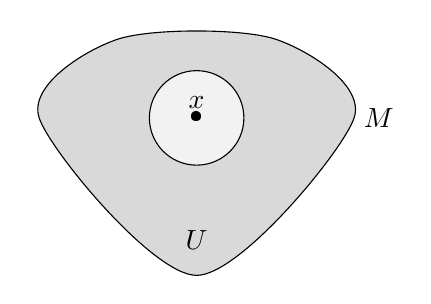
\begin{tikzpicture}
      \fill[gray!30] plot [smooth cycle] coordinates {(0,0) (1,1) (3,1) (4,0) (2,-2)};
      \draw plot [smooth cycle] coordinates {(0,0) (1,1) (3,1) (4,0) (2,-2)};
      \fill[gray!10] (2,0) circle (0.6);
      \node () at (2,0) {\textbullet};
      % \node[right] () at (2.6,0) {$ V $};
      \node[above] () at (2,0) {$ x $};
      \draw (2,0) circle (0.6);
      \node[above] () at (2,-1.8) {$ U $};
      \node[right] () at (4,0) {$ M $};
    \end{tikzpicture}
    \caption{Situazione}
    \label{fig:lez13:dimension_topological_invariance}
  \end{figure}
  L'immersione di $ \Disk{m} \setminus \set{\vec{0}} $ in $ \Disk{m} $ induce una
  successione esatta lunga in omologia relativa ridotta, da cui si trova
  facilmente che:
  \[
    H_i(\Disk{m}, \Disk{m} \setminus \set{\vec{0}}) \cong \tilde{H}_{i-1}(\Disk{m} \setminus \set{\vec{0}})
  \]
  Ma $ \Disk{m} \setminus \set{\vec{0}} \sim_h \Sph{m-1} $ quindi
  $ \tilde{H}_i(\Disk{m} \setminus \set{\vec{0}}) \cong \tilde{H}_i(\Sph{m-1}) $
  e perciò:
  \[
    H_i(M, M \setminus \set{x}) \cong \tilde{H}_i(\Sph{m-1})
  \]
  A questo punto diventa semplice collegare due varietà differenti: se $ M \simeq N $
  allora:
  \[
    H_i(M, M \setminus \set{x}) \cong H_i(N, N \setminus \set{y})
  \]
  Cioè:
  \[
    \tilde{H}_i(\Sph{m-1}) \cong \tilde{H}_i(\Sph{n-1})
  \]
  Quindi necessariamente $ m = n $.
\end{proof}
\begin{osservation}
  Non vale il viceversa, come ad esempio un toro e una sfera, che hanno la stessa
  dimensione topologica ma non sono omeomorfi.
\end{osservation}

%%% Local Variables:
%%% mode: latex
%%% TeX-master: "notes"
%%% End:
